\documentclass[12pt,a4paper]{article}

\usepackage[a4paper,margin=1.15in]{geometry}
\usepackage{graphicx}
\graphicspath{{figures/}}
\usepackage{booktabs}
\usepackage{array}
\usepackage{amsmath}
\usepackage{amssymb}
\usepackage{float}
\usepackage{subcaption}
\usepackage{xcolor}
\usepackage{enumitem}
\usepackage{multirow}
\usepackage{caption}
\usepackage{microtype}
\usepackage[colorlinks=true,linkcolor=blue!50!black,citecolor=blue!50!black,urlcolor=blue!50!black]{hyperref}
\usepackage{setspace}
\onehalfspacing

\setlength{\parskip}{5pt}
\captionsetup{font=small,labelfont=bf}
\newcommand{\pbrk}{\discretionary{}{}{}}

\title{\textbf{CrisisSense: Crisis Language Detection Using NLP}}
\author{CrisisSense Project}
\date{September 2026}

\begin{document}
\maketitle
\vspace{-0.4cm}

\noindent CrisisSense is a frozen, three-class text-classification system that compares two independently trained models --- character-level TF-IDF with Logistic Regression, and a locally hosted BERT sequence classifier --- on the same submitted text, and displays both predictions side by side without combining them into an ensemble. On a shared 195-row frozen test set, BERT reaches higher overall accuracy (76.92\% vs.\ 71.28\%) and macro-F1 (74.66\% vs.\ 69.62\%), while TF-IDF + Logistic Regression is marginally ahead on the implicit-crisis class specifically (67.92\% vs.\ 67.33\% F1). BERT's mean confidence (94.60\%) is far higher than TF-IDF's (55.74\%), but its Expected Calibration Error (0.177) is also higher, not lower, than TF-IDF's (0.155). The two models agree on 75.9\% of test examples. CrisisSense classifies crisis-related language in text; it is not a clinical diagnostic system and does not assess suicide risk.

\section{Introduction}

\subsection{Background}

Crisis-related language on text platforms rarely takes one shape. Some statements name crisis intent directly; others convey the same meaning indirectly, through understatement, metaphor, or context that has to be inferred rather than matched. A detection system built only on keyword matching reliably catches the former and largely misses the latter, while a system with no lexical grounding at all may over-generalize from superficial similarity. This tension motivates CrisisSense, which treats crisis-language detection as a three-class problem and studies how two structurally different models --- a sparse character-level lexical model and a contextual transformer --- perform on the same task and the same data.

\subsection{Problem Statement}

Given a piece of submitted text, CrisisSense assigns one of three labels: \texttt{no\_crisis} (class 0), text that does not indicate crisis-related language; \texttt{implicit\_crisis} (class 1), crisis-related meaning expressed indirectly rather than as a direct statement; and \texttt{explicit\_crisis} (class 2), crisis-related language expressed directly. This is a single-label, three-class classification problem over free text --- not a four-class or severity-graded problem, not a clinical risk-assessment task, and not a generative task.

\subsection{Motivation}

Implicit crisis language is the harder and arguably more consequential case: it is the category most likely to be missed by naive keyword filters, yet it is also the category with the fewest unambiguous lexical cues to exploit. Comparing a lexical, character-level model against a contextual transformer on the same frozen test set makes it possible to ask a concrete empirical question --- does additional contextual modeling capacity actually help on the implicit-crisis class specifically, or only on the classification task in aggregate --- rather than relying on the intuition that ``bigger models are strictly better.''

\subsection{Objectives and Scope}

The system (1) builds a reproducible, frozen three-class dataset split with verified class balance and no duplicate rows; (2) trains and freezes a character-level TF-IDF + Logistic Regression baseline; (3) loads and evaluates a BERT sequence-classification model as a frozen, inference-only artifact; (4) evaluates both models on an identical held-out test set across accuracy, per-class F1, confidence, calibration, and agreement; and (5) serves both models independently, side by side, without combining their outputs into an ensemble.

CrisisSense is explicitly \emph{not} a four-class or severity-graded system, not a clinical risk-assessment tool, and not an ensemble. The repository also retains historical four-class annotation material (with a separate \texttt{hard\_negative} label) and unused Word2Vec code; neither is part of the current deployed system, and neither is used anywhere in this report.

\subsection{Contributions}

\begin{enumerate}[nosep]
  \item A reproducible, frozen three-class dataset split (905/194/195 rows) with verified zero cross-split duplication.
  \item A fully specified character-level TF-IDF + Logistic Regression pipeline, evaluated end to end on the shared test set.
  \item A fully specified BERT sequence-classification pipeline (12-layer, 768-hidden, 12-head, 3-label), evaluated as a frozen inference-only artifact.
  \item A side-by-side comparison covering overall metrics, per-class metrics, confusion matrices, confidence, Expected Calibration Error, and inter-model agreement.
  \item An explicit boundary separating the current three-class deployed system from historical four-class and Word2Vec-based research material retained elsewhere in the repository.
\end{enumerate}

\section{Related Work}

\textbf{Crisis language detection.} Automatic detection of crisis- and suicide-related language is commonly framed as text classification over social-media posts, forum text, or clinical notes. A recurring difficulty is that crisis intent is frequently not stated in keyword-matchable form; language can convey the same underlying state through indirection, metaphor, or understatement. This motivates treating implicit and explicit expression as distinct classes rather than a single binary crisis/no-crisis label, which is the design choice CrisisSense makes.

\textbf{Traditional NLP classification.} Before pretrained transformer encoders, text classification was dominated by sparse, feature-based pipelines: a document is mapped to a high-dimensional numeric vector, and a linear or shallow classifier is fit on top. These pipelines remain competitive baselines because they are inexpensive to train, fast at inference, and behave predictably on noisy or out-of-distribution text.

\textbf{TF-IDF and linear models.} TF-IDF weighting~\cite{sparckjones1972statistical} scores a term by how often it appears in a document relative to how common it is corpus-wide, so terms frequent everywhere contribute little discriminative signal. Logistic Regression~\cite{cox1958regression} is the standard linear classifier paired with TF-IDF features. Character-level n-gram variants are particularly relevant for informal or misspelled text, since they degrade gracefully under spelling variation rather than requiring a fixed whole-word vocabulary.

\textbf{Transformer-based classification and BERT.} The Transformer~\cite{vaswani2017attention} replaced recurrence with self-attention, letting every token attend to every other token directly. BERT~\cite{devlin2019bert} is a bidirectional pretrained encoder producing contextual token representations. \texttt{BertForSequenceClassification} attaches a linear head to its pooled output --- the architecture used by CrisisSense's BERT artifact --- implemented through Hugging Face Transformers~\cite{wolf2020transformers} on PyTorch~\cite{paszke2019pytorch}.

\textbf{Comparison and calibration.} Contextual models are generally expected to outperform sparse baselines on tasks requiring disambiguation from context, but this advantage need not be uniform across every subclass of a task: a model can improve overall accuracy while leaving a harder, pragmatically defined subclass largely unchanged. Neural classifiers, including fine-tuned transformers, are also repeatedly shown to be poorly calibrated~\cite{guo2017calibration,naeini2015obtaining}: softmax confidence does not reliably track the true probability of correctness. This is directly relevant to CrisisSense's BERT model, which produces much higher confidence than TF-IDF without a proportional improvement in calibration.

\textbf{Research gap.} Much applied work on crisis-language detection reports a single model's aggregate accuracy without separating overall performance from class-specific performance, and without jointly reporting confidence, calibration, and inter-model agreement as distinct axes. This report evaluates two structurally different models on identical data and reports all of these axes separately rather than collapsing them into one headline number.

\section{Data and Dataset Analysis}

\subsection{Value of the Data}

\begin{itemize}[nosep]
  \item \textbf{Total samples.} 1{,}294 rows total, split 905/194/195 (train/validation/test), stratified, seed 42.
  \item \textbf{Label construction.} Labels are collapsed from an original ordinal \texttt{severity} field (0--6): severity 0 $\rightarrow$ \texttt{no\_crisis}; severity 1 $\rightarrow$ \texttt{implicit\_crisis}; severity 2--6 $\rightarrow$ \texttt{explicit\_crisis}.
  \item \textbf{Provenance.} The three split files are explicit, byte-preserved copies of \texttt{experiments/\pbrk tfidf\_baseline/\pbrk results/\pbrk data\_split.csv}, filtered by its existing \texttt{split} column; no resampling or re-partitioning was performed, and row order, text, and labels are unchanged from the source.
  \item \textbf{Audit.} Zero duplicate rows, zero duplicate \texttt{content} values, zero cross-split overlap, and no blank \texttt{content}/\texttt{label} values across all 1{,}294 rows.
  \item \textbf{Evaluation set.} Both models are evaluated on exactly the same 195-row \texttt{test.csv}, so every result in Section~7 is directly comparable across models.
\end{itemize}

\subsection{Label Definitions and Dataset Statistics}

\begin{table}[H]
\centering
\caption{Current class definitions.}
\begin{tabular}{clp{7.5cm}}
\toprule
\textbf{ID} & \textbf{Class} & \textbf{Meaning} \\
\midrule
0 & \texttt{no\_crisis} & Text that does not indicate crisis-related language. \\
1 & \texttt{implicit\_crisis} & Crisis-related meaning expressed indirectly. \\
2 & \texttt{explicit\_crisis} & Crisis-related language expressed directly. \\
\bottomrule
\end{tabular}
\end{table}

\begin{table}[H]
\centering
\caption{Class distribution across the frozen splits.}
\begin{tabular}{lrrrr}
\toprule
\textbf{Split} & \textbf{No Crisis} & \textbf{Implicit} & \textbf{Explicit} & \textbf{Total} \\
\midrule
Train      & 245 & 227 & 433 & 905 \\
Validation & 53  & 48  & 93  & 194 \\
Test       & 53  & 49  & 93  & 195 \\
\midrule
\textbf{Total} & \textbf{351} & \textbf{324} & \textbf{619} & \textbf{1{,}294} \\
\bottomrule
\end{tabular}
\end{table}

Explicit-crisis is the plurality class (\textasciitilde48\%) in every split; no-crisis and implicit-crisis are more evenly matched (\textasciitilde27\% and \textasciitilde25\%). Because the split is stratified, this proportion is preserved from training through to test.

\subsection{Dataset Limitations}

The test split contains only 195 rows, of which 49 (25.1\%) belong to implicit-crisis --- the class most central to this project's motivation and also the smallest of the three. Metrics computed on 49 implicit-crisis examples carry a wider margin of statistical uncertainty than the corresponding explicit-crisis metrics, computed on 93 examples. The dataset's original annotation methodology is not independently re-verifiable from the current runtime artifacts alone.

\section{Methodology}

\subsection{System Architecture}

CrisisSense is a single FastAPI process that both serves a static frontend and exposes \texttt{POST /predict}. Submitted text is routed independently to the frozen TF-IDF/Logistic Regression pipeline and the frozen BERT pipeline; neither path fits, refits, or writes to a model artifact at request time, and their outputs are never combined into a single ensemble prediction.

\begin{figure}[H]
\centering
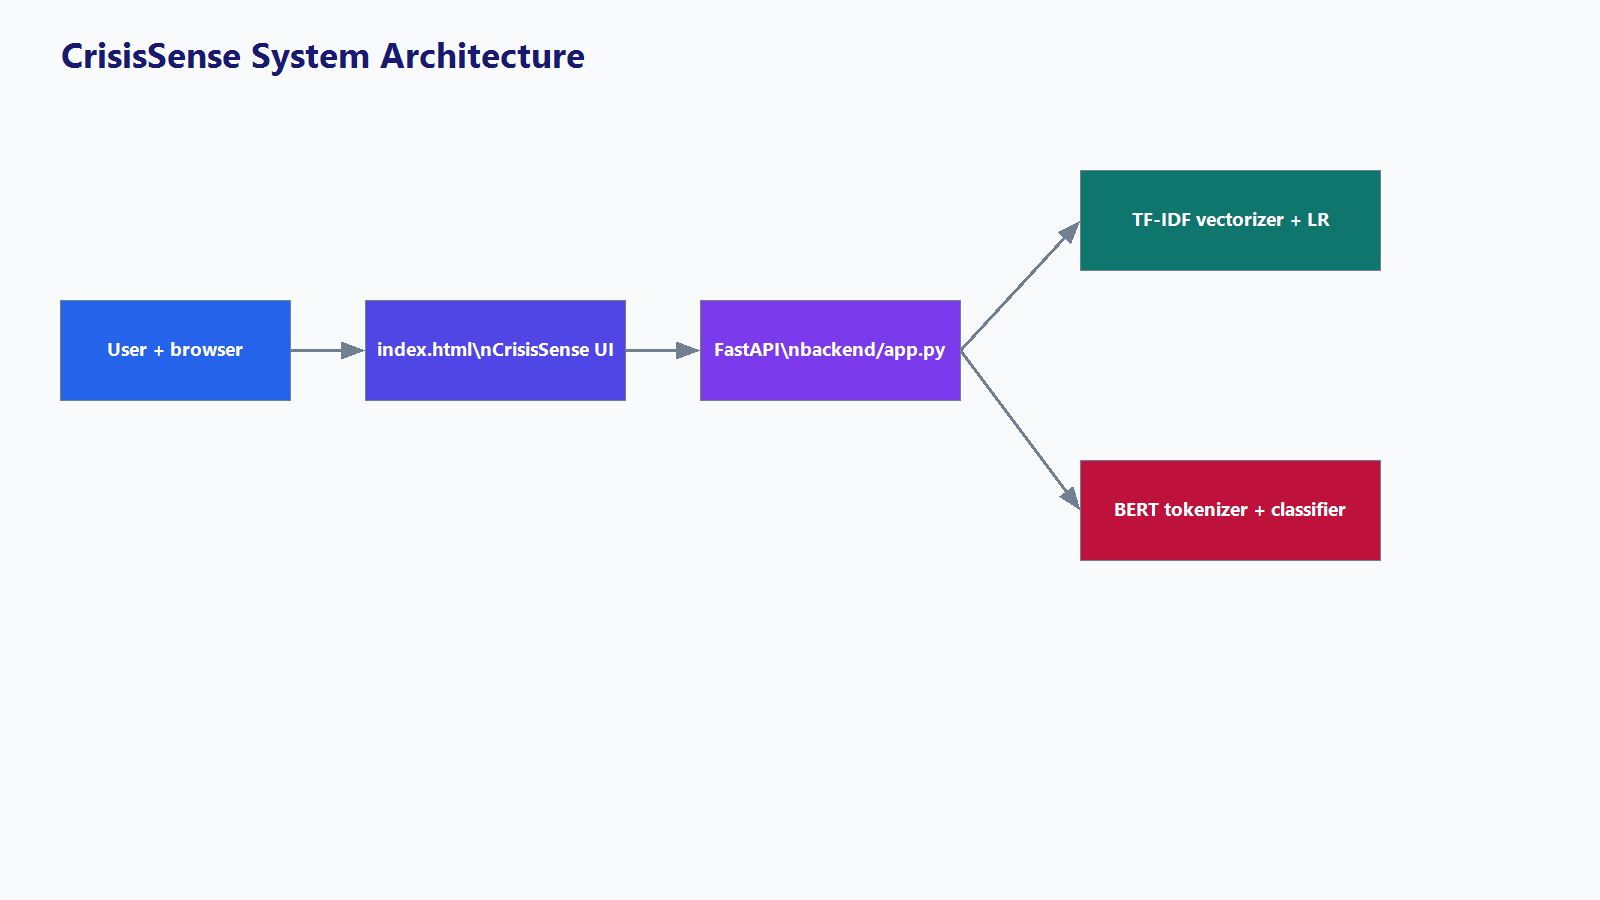
\includegraphics[width=0.8\textwidth]{system-architecture.png}
\caption{Overall system architecture: independent TF-IDF and BERT paths behind a single FastAPI \texttt{/predict} endpoint.}
\end{figure}

\begin{figure}[H]
\centering
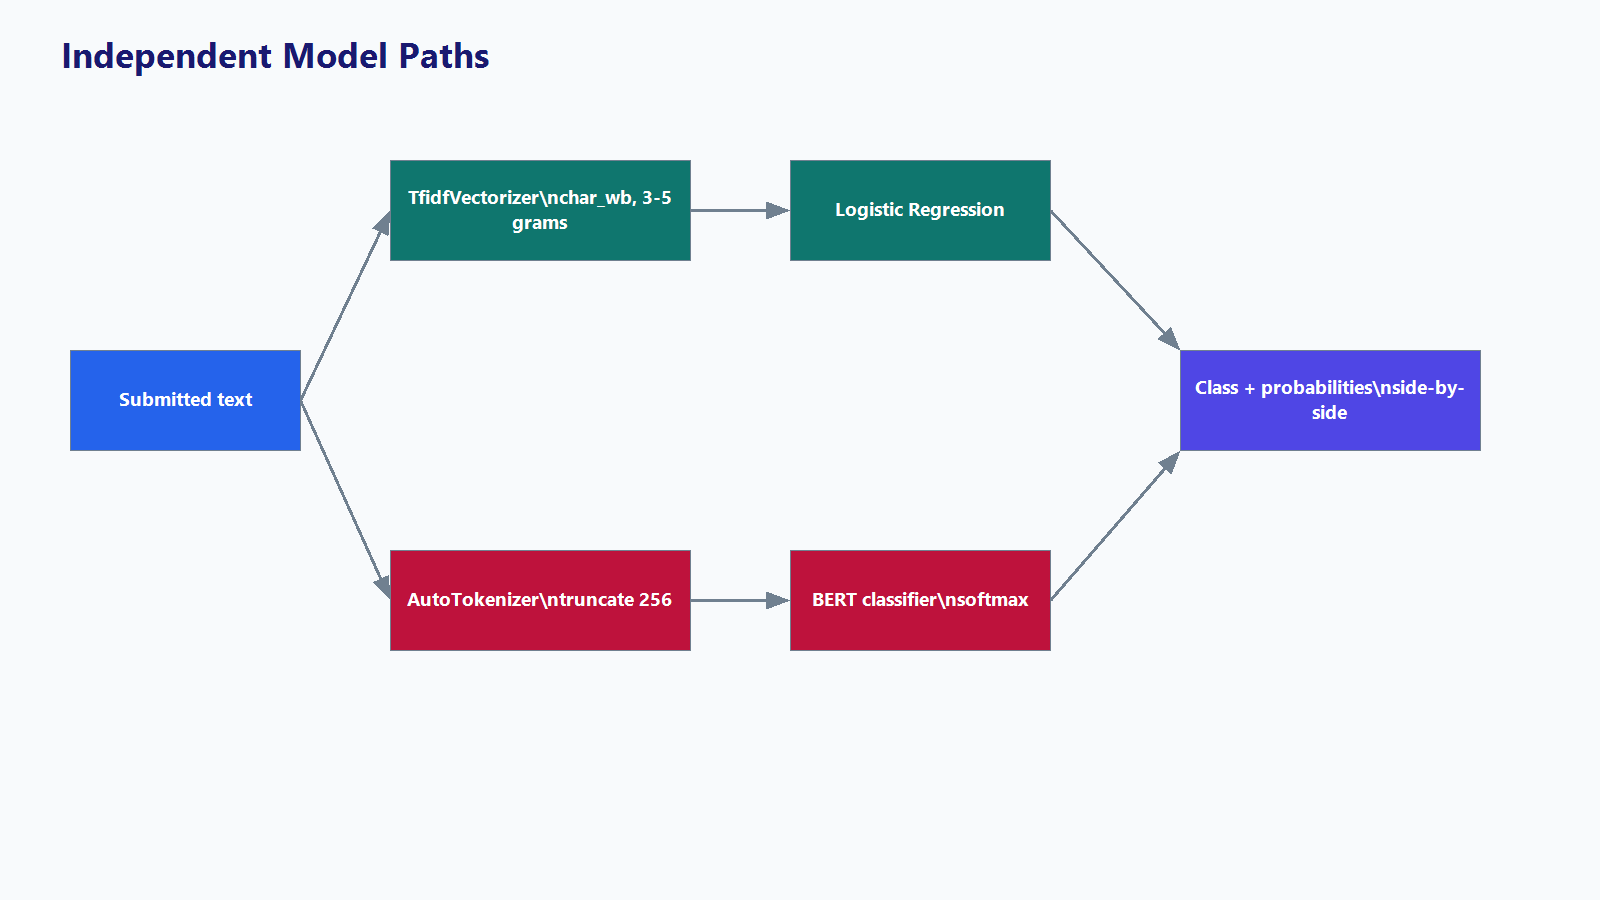
\includegraphics[width=0.8\textwidth]{model-comparison.png}
\caption{Independent model paths. Submitted text is processed separately by the TF-IDF + Logistic Regression pipeline and the BERT pipeline; both are displayed together without being combined.}
\end{figure}

\begin{figure}[H]
\centering
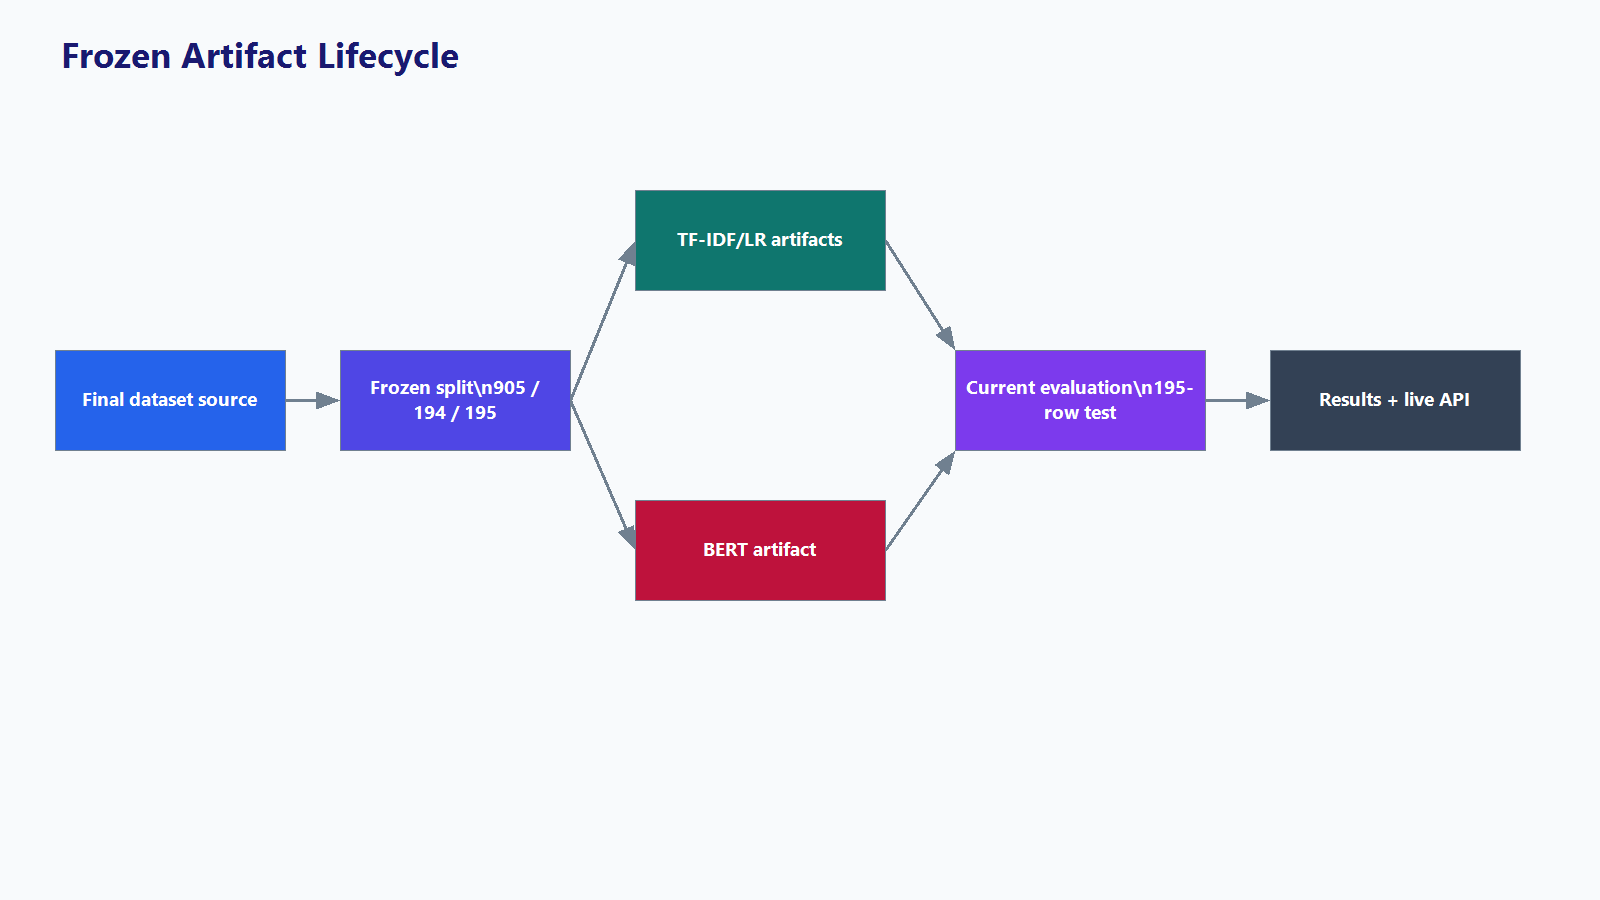
\includegraphics[width=0.8\textwidth]{artifact-lifecycle.png}
\caption{Frozen artifact lifecycle: the same TF-IDF/LR and BERT artifacts feed both offline evaluation and live inference; neither path fits, refits, or overwrites the artifacts.}
\end{figure}

\subsection{TF-IDF + Logistic Regression}

The frozen vectorizer uses a \texttt{char\_wb} analyzer (character n-grams within word boundaries, range 3--5), \texttt{min\_df}=2, \texttt{max\_df}=0.9, sublinear term-frequency scaling, \texttt{max\_features}=50{,}000, lowercasing, and Unicode accent stripping, producing 17{,}708 fitted features on the training split only. At inference time the backend calls \texttt{vectorizer.transform([text])} directly on raw text --- no separate stop-word removal, stemming, or URL/punctuation stripping occurs beyond what the vectorizer itself performs.

Term frequency--inverse document frequency weights a term $t$ in document $d$ as
\begin{equation}
\mathrm{TFIDF}(t,d) = \mathrm{TF}(t,d)\times\mathrm{IDF}(t), \qquad \mathrm{IDF}(t)=\ln\!\left(\frac{N}{n_t}\right),
\end{equation}
where $N$ is the corpus size and $n_t$ the number of documents containing $t$. The resulting sparse vector is passed to a multinomial Logistic Regression classifier ($C{=}1.0$, \texttt{class\_weight=balanced}, \texttt{lbfgs}, \texttt{max\_iter}=5000, seed 42):
\begin{equation}
P(y=k\mid x) = \frac{\exp(w_k^\top x + b_k)}{\sum_{j=1}^{3}\exp(w_j^\top x + b_j)}.
\end{equation}
The balanced class-weight setting reweights the training loss inversely to class frequency, compensating for the moderate imbalance in Table~2.

\subsection{BERT}

The frozen BERT artifact is a standard \texttt{BertForSequenceClassification} (12 layers, hidden size 768, 12 attention heads, vocabulary 30{,}522, 3 output labels), loaded locally with \texttt{local\_files\_only=True} so no network call to a model hub occurs. Text is tokenized, truncated to 256 tokens, and passed through the encoder under \texttt{torch.inference\_mode()}. Each layer computes scaled dot-product self-attention,
\begin{equation}
\mathrm{Attention}(Q,K,V) = \mathrm{softmax}\!\left(\frac{QK^\top}{\sqrt{d_k}}\right)V,
\end{equation}
letting every token's representation update using information from every other token in the sequence. The pooled representation of the final layer is mapped by a linear classification head to three logits $z$, converted to class probabilities by softmax,
\begin{equation}
P(y=k\mid x) = \frac{\exp(z_k)}{\sum_{j=1}^{3}\exp(z_j)}.
\end{equation}
This report evaluates the already-trained, saved BERT artifact as deployed; its original fine-tuning process is not re-executed or re-verified here.

\subsection{Model Comparison}

\begin{table}[H]
\centering
\caption{Structural comparison of the two independent model paths.}
\begin{tabular}{lll}
\toprule
\textbf{Property} & \textbf{TF-IDF + Logistic Regression} & \textbf{BERT} \\
\midrule
Representation & Character-boundary TF-IDF & Contextual transformer \\
Classifier & Logistic Regression & Sequence-classification head \\
Artifact & Two \texttt{.joblib} files & Local weights, tokenizer, config \\
Runtime & scikit-learn, CPU & CUDA if available, else CPU \\
Relationship & \multicolumn{2}{c}{Independent --- never combined} \\
\bottomrule
\end{tabular}
\end{table}

\section{Implementation}

\subsection{Software Stack}

\begin{table}[H]
\centering
\caption{Current software and environment stack.}
\begin{tabular}{ll}
\toprule
\textbf{Component} & \textbf{Library / Requirement} \\
\midrule
Language & Python 3.10+ \\
Web framework & FastAPI ($\geq$0.116), Uvicorn ($\geq$0.35) \\
Classical ML & scikit-learn ($\geq$1.3)~\cite{pedregosa2011scikit}, joblib ($\geq$1.3) \\
Deep learning & PyTorch ($\geq$2.0)~\cite{paszke2019pytorch}, Transformers ($\geq$4.35)~\cite{wolf2020transformers} \\
Frontend & Static HTML (\texttt{index.html}) with Tailwind CSS via CDN \\
Artifact versioning & Git LFS (tracks \texttt{.joblib} and BERT weight files) \\
\bottomrule
\end{tabular}
\end{table}

\subsection{Backend and API Endpoints}

The backend, \texttt{backend/\pbrk app.py}, loads both frozen model artifacts once at FastAPI startup, inside a \texttt{lifespan} context manager; if loading fails, \texttt{/health} and \texttt{/predict} respond with HTTP 503 rather than a fabricated prediction. Every request served afterward reuses the same in-memory model objects.

\begin{table}[H]
\centering
\caption{Current backend API endpoints.}
\begin{tabular}{lp{9.3cm}}
\toprule
\textbf{Endpoint} & \textbf{Purpose} \\
\midrule
\texttt{GET /} & Serves \texttt{index.html}. \\
\texttt{GET /health} & Reports model load status; HTTP 503 if artifacts failed to load. \\
\texttt{GET /project-info} & Reads current split row counts; returns totals and class count. \\
\texttt{GET /evaluation/\{filename\}} & Serves only the three frontend-approved evaluation graphs. \\
\texttt{POST /predict} & Accepts \texttt{\{"text": "..."\}}; returns independent TF-IDF and BERT results. Blank text is rejected with HTTP 422. \\
\bottomrule
\end{tabular}
\end{table}

\subsection{Reproducibility}

\begin{quote}
\ttfamily\small
python -m venv .venv\\
.\textbackslash .venv\textbackslash Scripts\textbackslash Activate.ps1\\
pip install -r requirements-ml.txt\\
git lfs pull\\
python -m uvicorn backend.app:app --host 127.0.0.1 --port 8000
\end{quote}

After these steps the application is available at \texttt{http://127.0.0.1:8000/}; a single FastAPI process serves both the API and the static frontend. \texttt{git lfs pull} is required after cloning because the vectorizer, classifier, and BERT weight files are stored through Git LFS. This reproducibility claim covers inference with the already-frozen artifacts and offline evaluation via the evaluation script; it does not claim that BERT's original fine-tuning process is reproduced from this repository state.

\section{Experimental Setup}

\subsection{Evaluation Metrics}

Both models are scored on the shared 195-row test set with standard classification metrics,
\begin{equation}
\mathrm{Precision}=\frac{TP}{TP+FP},\quad \mathrm{Recall}=\frac{TP}{TP+FN},\quad F1=\frac{2\,\mathrm{Precision}\cdot\mathrm{Recall}}{\mathrm{Precision}+\mathrm{Recall}},
\end{equation}
macro-averaged across the three classes so that the smaller implicit-crisis class contributes equally to the aggregate score,
\begin{equation}
\mathrm{Macro\text{-}F1} = \tfrac{1}{3}\left(F1_{\text{no}} + F1_{\text{implicit}} + F1_{\text{explicit}}\right).
\end{equation}
A $3\times3$ confusion matrix is computed per model (rows = true label, columns = predicted label); its diagonal entries are correct predictions and its off-diagonal entries reveal \emph{which} classes a model confuses. Confidence is the selected-class probability $p_{\hat{y}}=\max_k P(y{=}k\mid x)$. Expected Calibration Error bins predictions by confidence and compares observed accuracy to mean confidence per bin,
\begin{equation}
\mathrm{ECE} = \sum_{b=1}^{B}\frac{n_b}{N}\left|\mathrm{acc}(b)-\mathrm{conf}(b)\right|.
\end{equation}
Agreement is the fraction of test rows where $\hat{y}_{\text{tfidf}}=\hat{y}_{\text{bert}}$, independent of correctness --- it measures consistency between the two independent classifiers, not correctness.

\subsection{Protocol}

\texttt{scripts/\pbrk evaluate\_\pbrk current\_\pbrk models.py} runs both frozen models through the same \texttt{FrozenModels} inference path used by the live API, over the identical 195-row \texttt{test.csv}, and writes metrics, a per-row prediction table, and figures to \texttt{results/\pbrk model\_\pbrk comparison/}. Using the identical inference path as the deployed API ensures the reported numbers describe the system as actually served, not a separately reimplemented evaluation pipeline.

\begin{figure}[H]
\centering
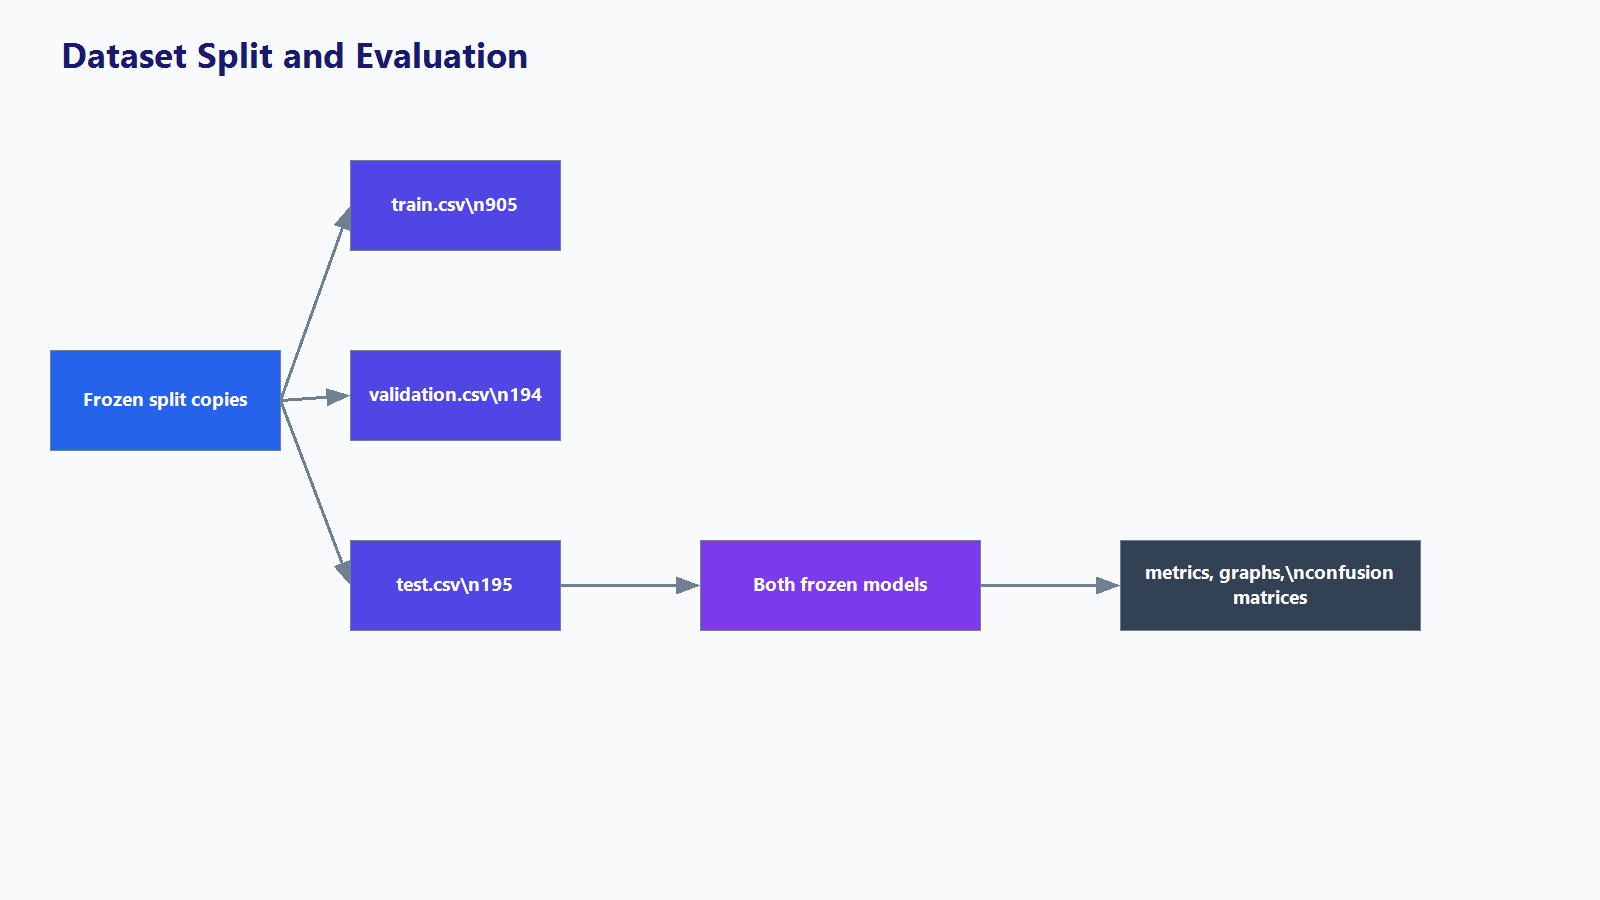
\includegraphics[width=0.75\textwidth]{dataset-evaluation.png}
\caption{Dataset-to-evaluation flow: the shared frozen test set feeds both frozen models identically; predictions are aggregated into metrics, confusion matrices, and presentation figures.}
\end{figure}

\begin{figure}[H]
\centering
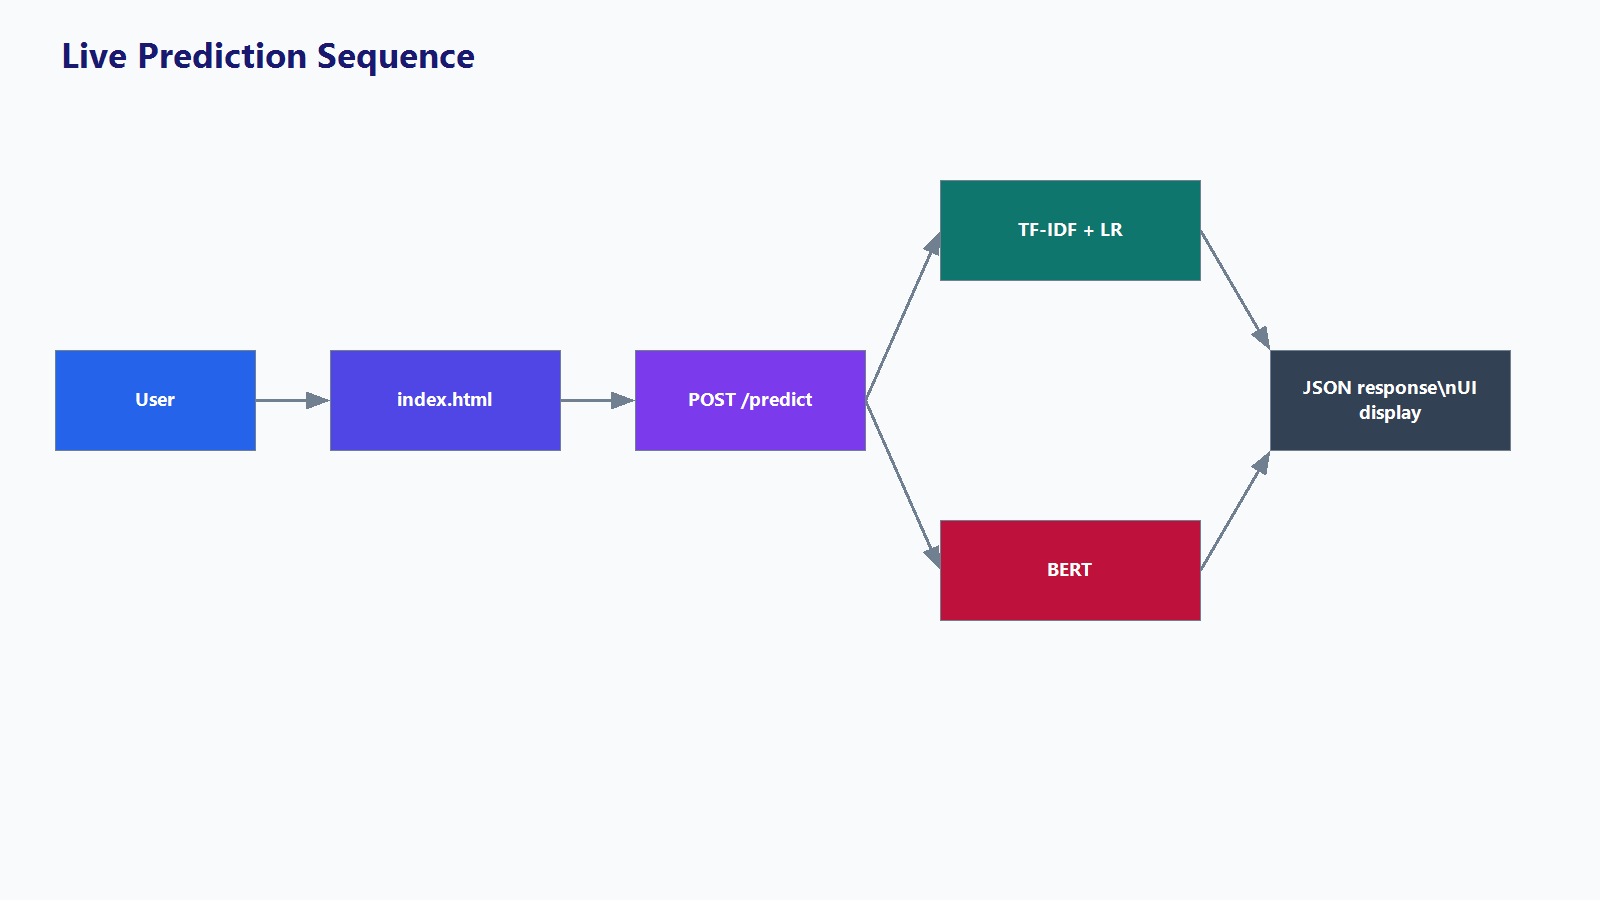
\includegraphics[width=0.75\textwidth]{live-prediction-sequence.png}
\caption{Live prediction sequence: a non-blank text submission triggers independent TF-IDF and BERT paths, whose results are returned together.}
\end{figure}

\section{Results and Discussion}

\subsection{Quantitative Results}

\begin{table}[H]
\centering
\caption{Overall test-set metrics (195 rows).}
\begin{tabular}{lrr}
\toprule
\textbf{Metric} & \textbf{TF-IDF + LR} & \textbf{BERT} \\
\midrule
Accuracy         & 71.28\% & 76.92\% \\
Macro Precision  & 70.07\% & 75.10\% \\
Macro Recall     & 69.79\% & 74.44\% \\
Macro F1         & 69.62\% & 74.66\% \\
\bottomrule
\end{tabular}
\end{table}

\begin{table}[H]
\centering
\caption{Per-class precision, recall, and F1.}
\begin{tabular}{llrrr}
\toprule
\textbf{Model} & \textbf{Class} & \textbf{Precision} & \textbf{Recall} & \textbf{F1} \\
\midrule
TF-IDF + LR & No Crisis  & 70.45\% & 58.49\% & 63.92\% \\
TF-IDF + LR & Implicit   & 63.16\% & 73.47\% & 67.92\% \\
TF-IDF + LR & Explicit   & 76.60\% & 77.42\% & 77.01\% \\
BERT        & No Crisis  & 76.60\% & 67.92\% & 72.00\% \\
BERT        & Implicit   & 65.38\% & 69.39\% & 67.33\% \\
BERT        & Explicit   & 83.33\% & 86.02\% & 84.66\% \\
\bottomrule
\end{tabular}
\end{table}

\begin{figure}[H]
\centering
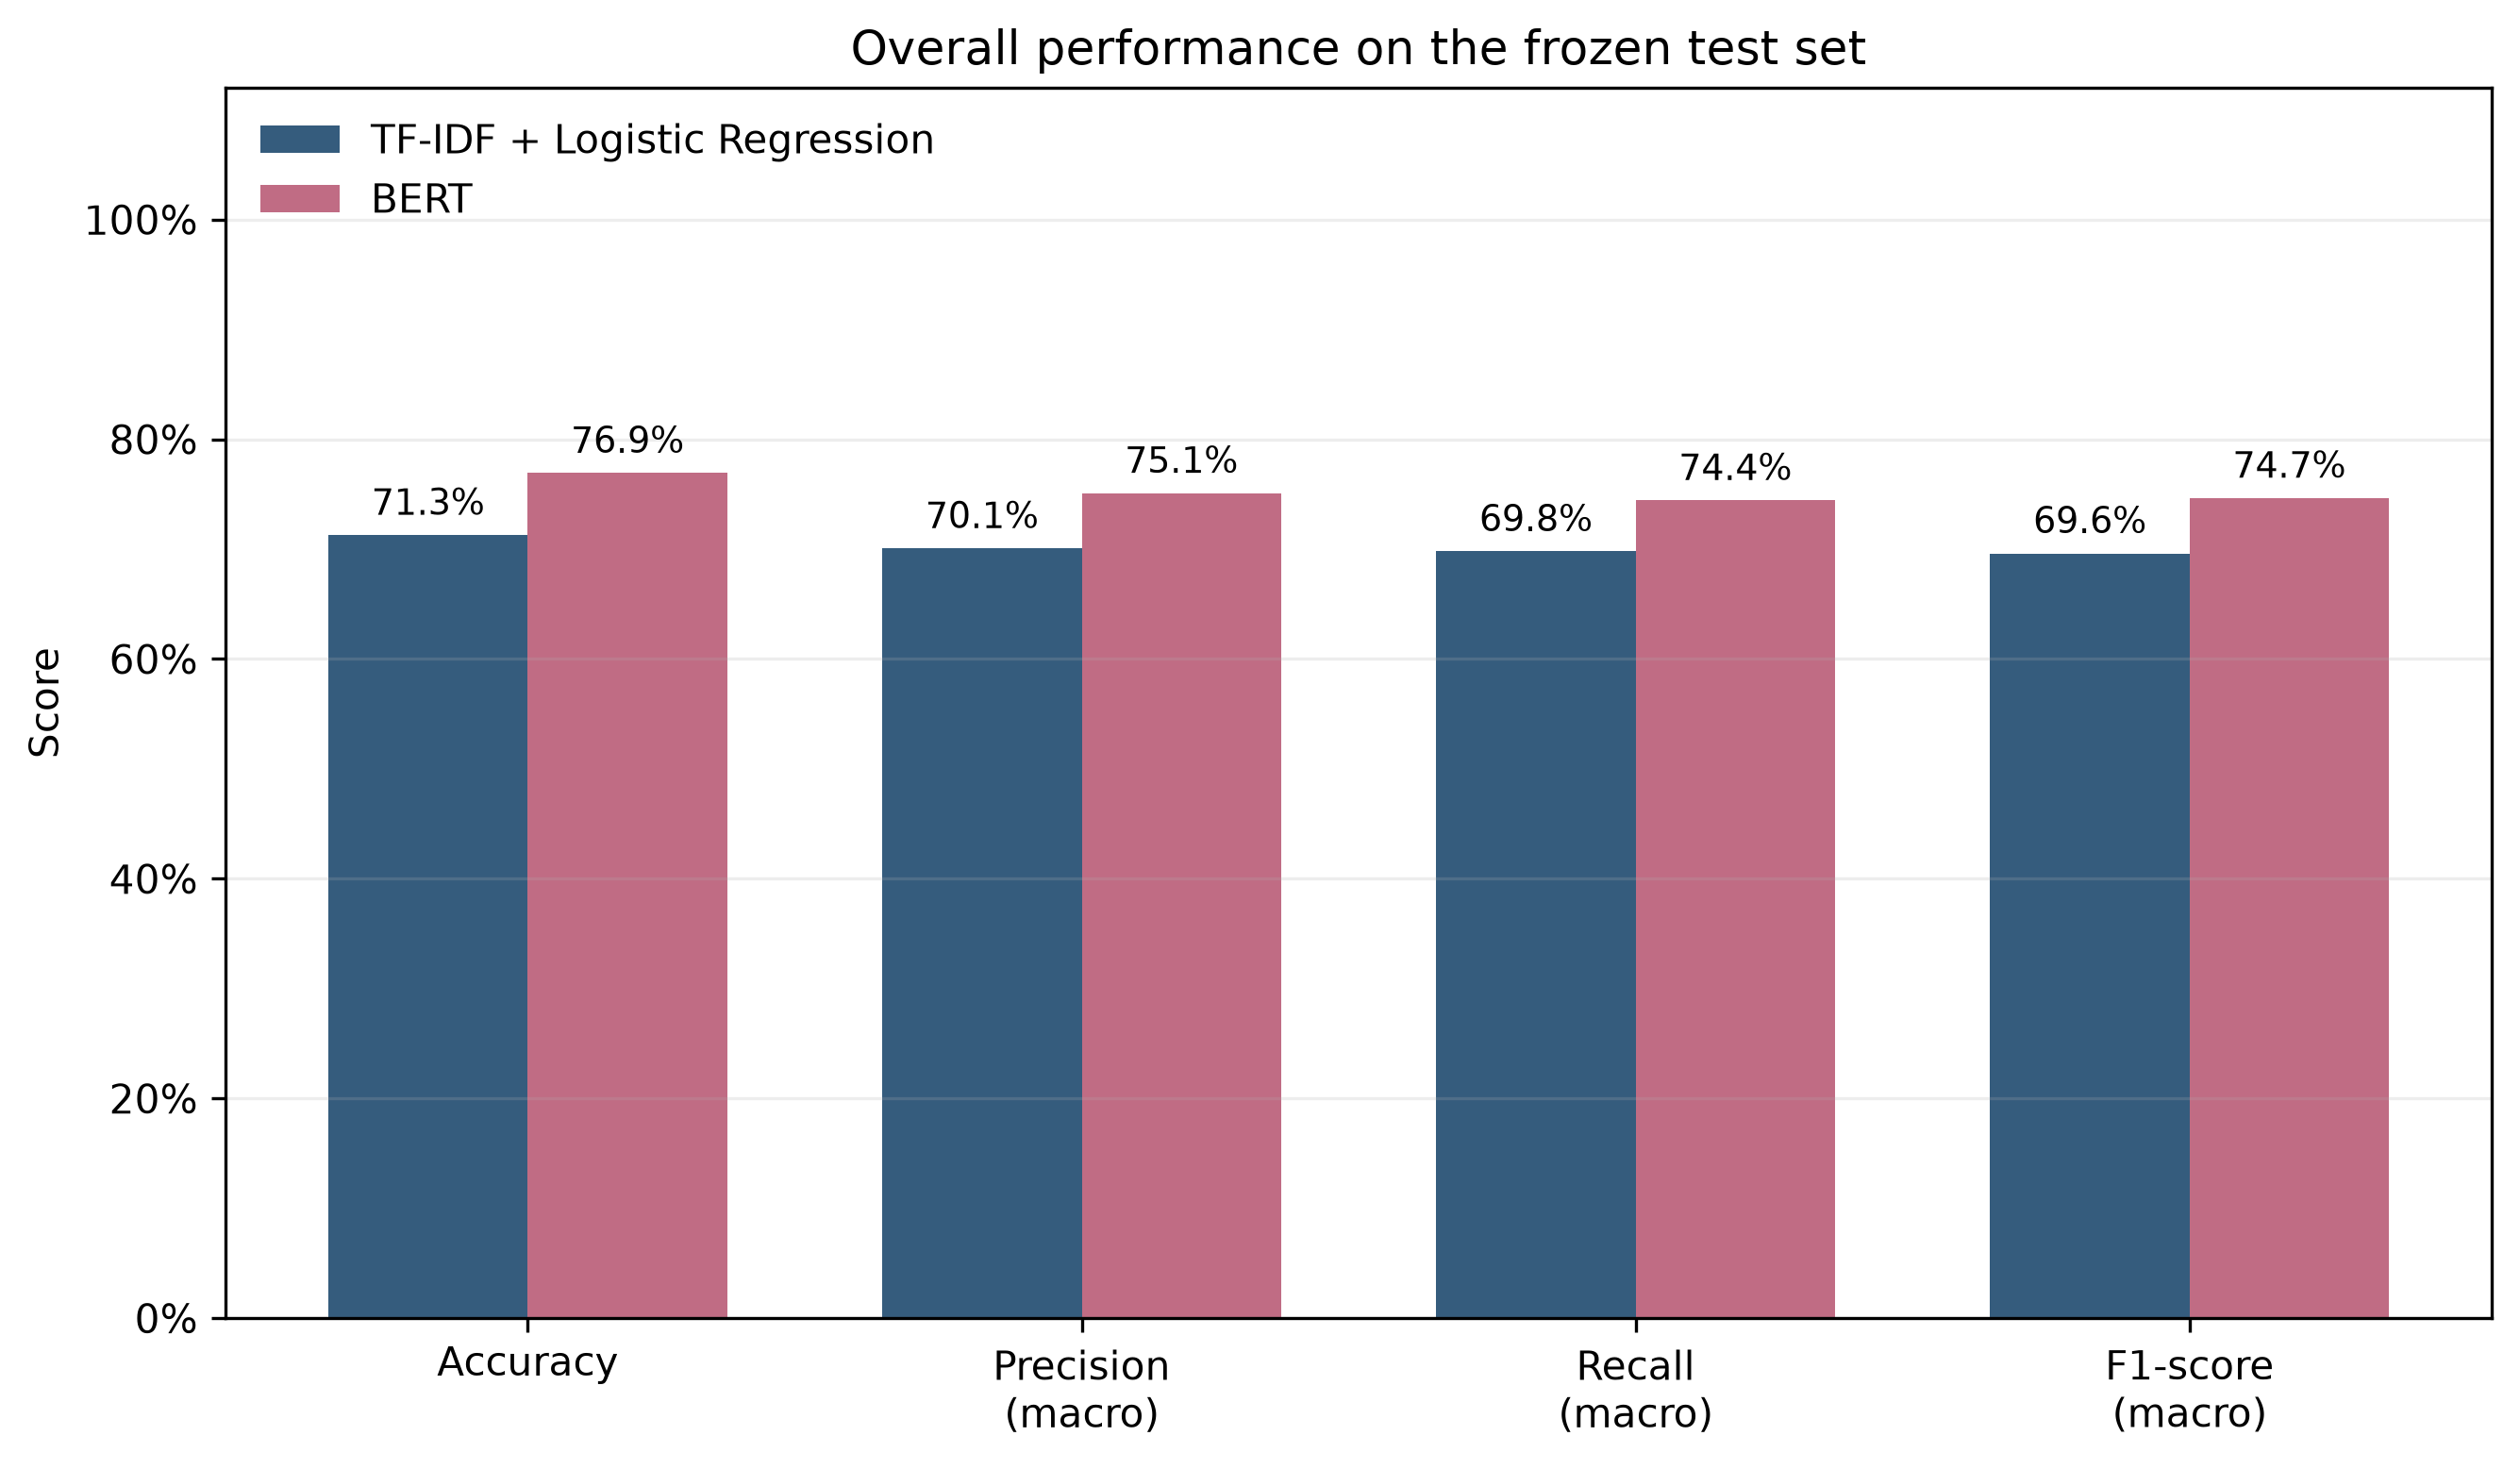
\includegraphics[width=0.75\textwidth]{overall_metrics.png}
\caption{Overall accuracy, macro precision, macro recall, and macro F1, TF-IDF + LR vs.\ BERT.}
\end{figure}

\begin{figure}[H]
\centering
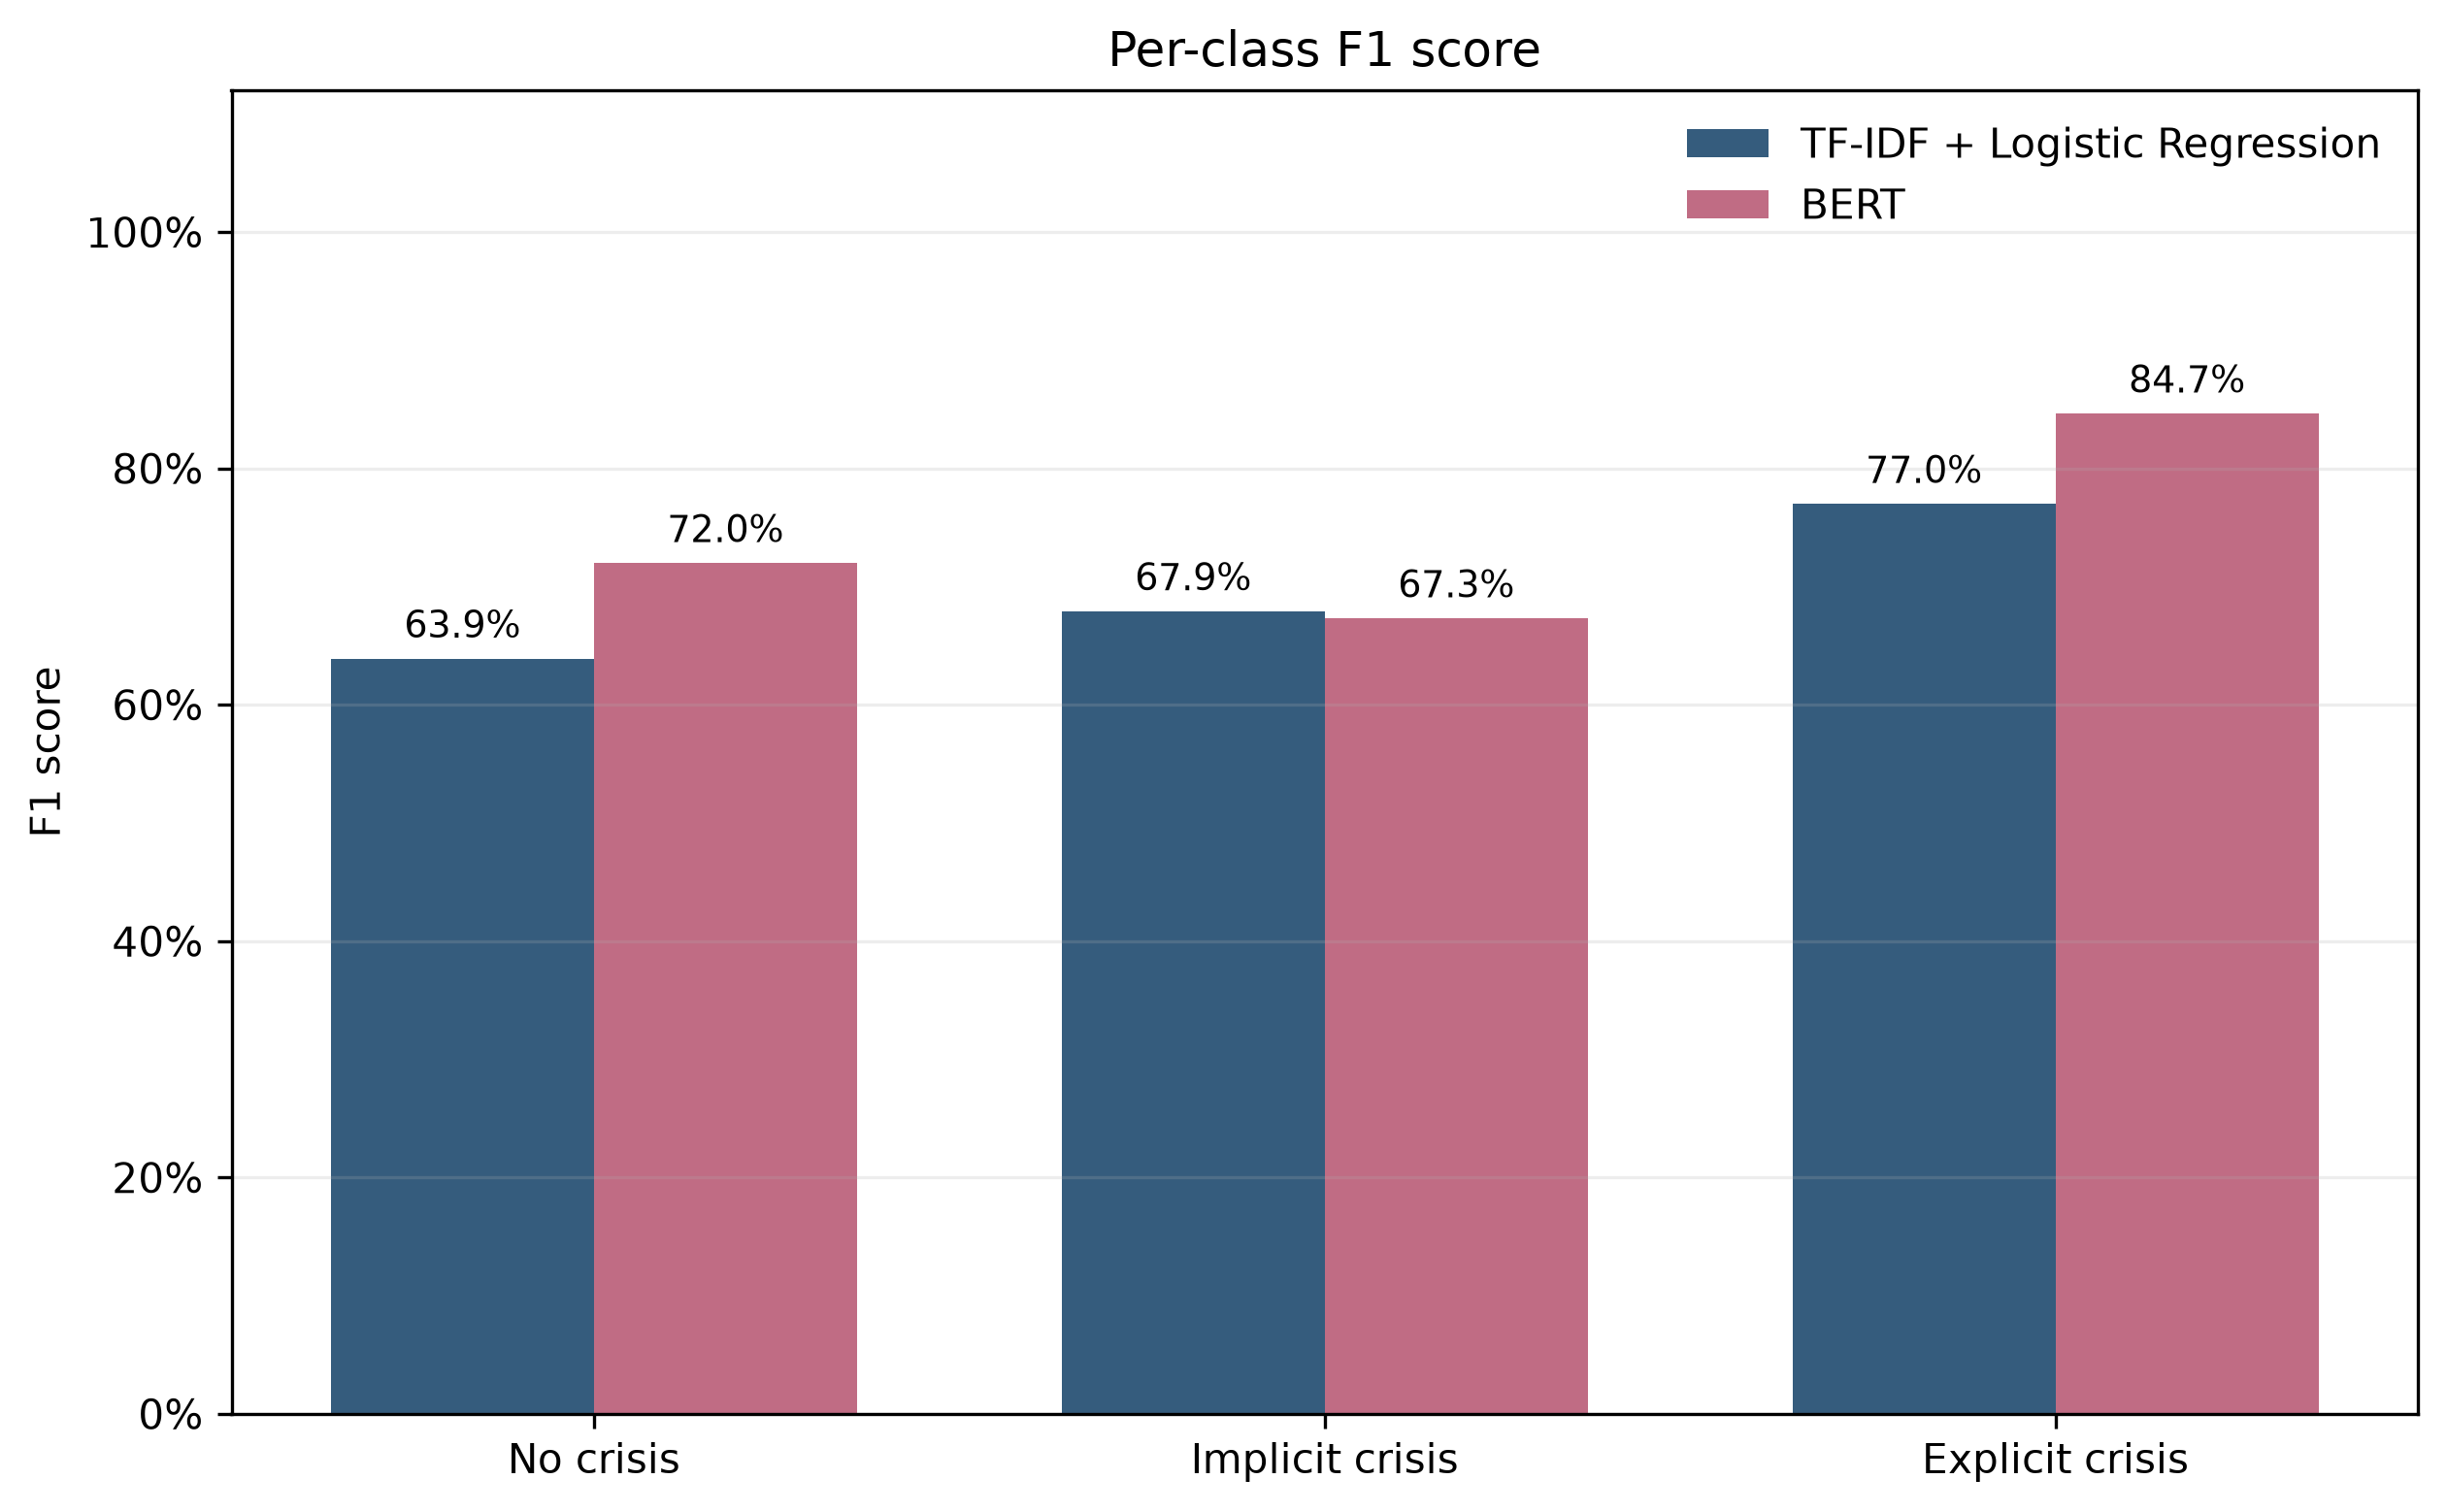
\includegraphics[width=0.75\textwidth]{per_class_f1.png}
\caption{Per-class F1 score for no-crisis, implicit-crisis, and explicit-crisis, by model.}
\end{figure}

BERT leads on every overall metric by 5--6 points and on explicit-crisis and no-crisis F1. On implicit-crisis, the two models are essentially tied, with TF-IDF marginally ahead (67.92\% vs.\ 67.33\% F1, on 49 test rows) --- the one class where this pattern reverses.

\subsection{Confusion Matrix Analysis}

\begin{figure}[H]
\centering
\begin{subfigure}[b]{0.48\textwidth}
\centering
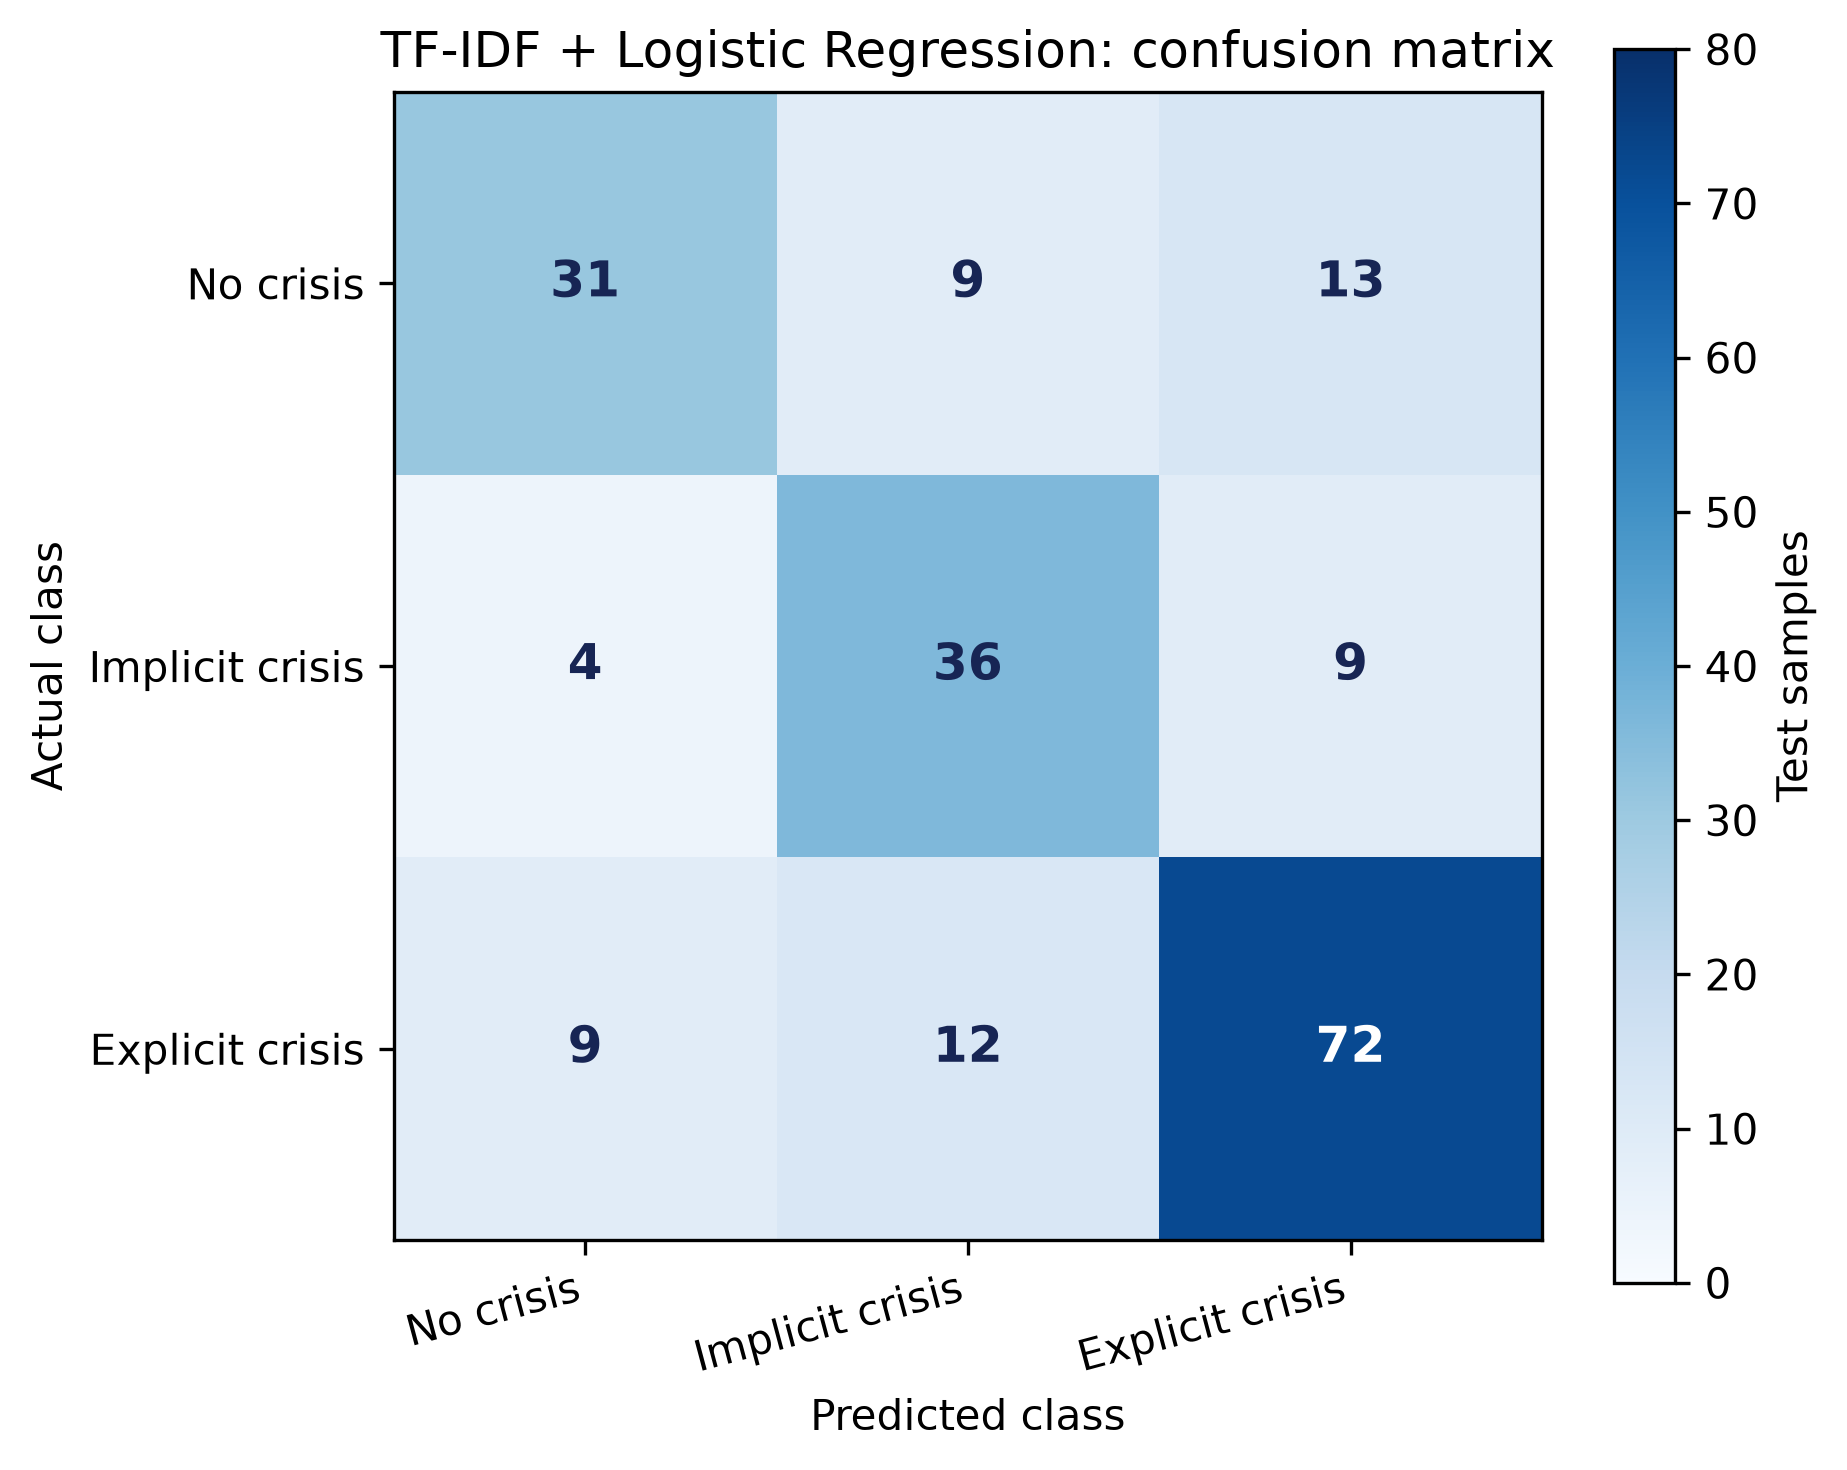
\includegraphics[width=\textwidth]{confusion_matrix_tfidf.png}
\caption{TF-IDF + LR}
\end{subfigure}
\hfill
\begin{subfigure}[b]{0.48\textwidth}
\centering
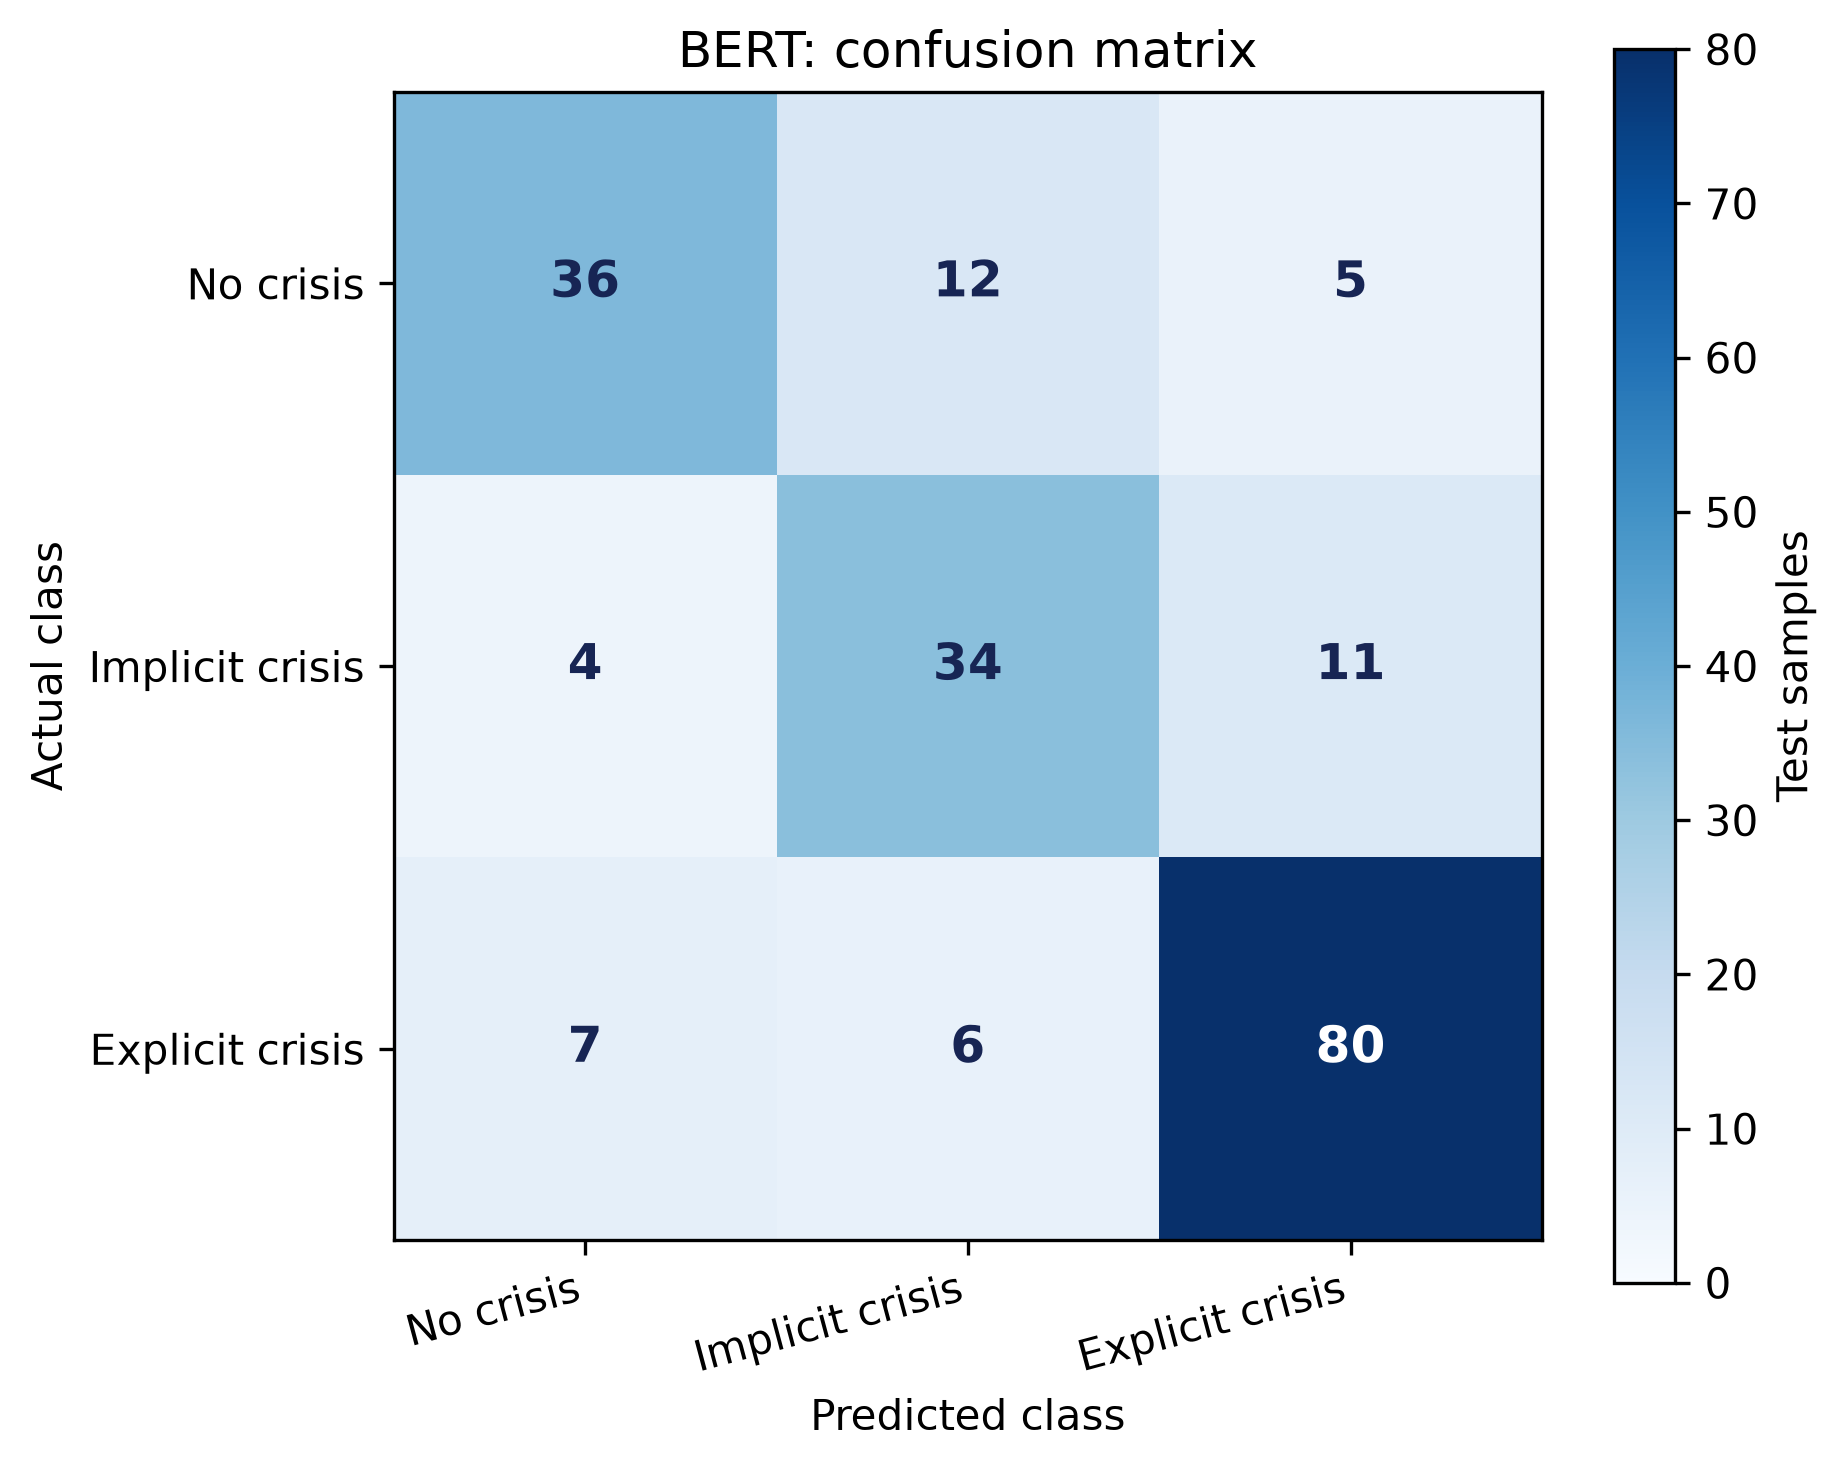
\includegraphics[width=\textwidth]{confusion_matrix_bert.png}
\caption{BERT}
\end{subfigure}
\caption{Confusion matrices on the shared 195-row test set (rows = actual, columns = predicted).}
\end{figure}

Both models place the largest diagonal mass on explicit-crisis (TF-IDF: 72/93 correct; BERT: 80/93). TF-IDF misclassifies 13 of 53 no-crisis rows as explicit-crisis, versus 5 of 53 for BERT --- BERT is markedly less prone to this specific error. On the implicit-crisis row, both models make 4 implicit$\rightarrow$no-crisis errors, but BERT makes more implicit$\rightarrow$explicit errors (11 vs.\ 9), meaning BERT is slightly more likely than TF-IDF to over-read implicit language as explicit.

\subsection{Implicit-, Explicit-, and No-Crisis Performance}

\textbf{Implicit-crisis} is the class this project is most concerned with and the class on which the two models are closest. TF-IDF's F1 (67.92\%) is driven by higher recall (73.47\% vs.\ BERT's 69.39\%) but lower precision (63.16\% vs.\ 65.38\%) than BERT. With only 49 test examples, this difference should be read as \emph{approximately tied} rather than a meaningful advantage for either model.

\textbf{Explicit-crisis} is where BERT shows its largest advantage: 84.66\% F1 versus 77.01\%, a 7.65-point gap driven by improvements in both precision and recall, on the largest of the three classes (93 examples).

\textbf{No-crisis} performance also favors BERT (72.00\% vs.\ 63.92\% F1), driven mainly by higher recall (67.92\% vs.\ 58.49\%): TF-IDF misclassifies a larger share of genuinely non-crisis text as crisis-related than BERT does.

\subsection{Confidence Distribution and Calibration}

\begin{table}[H]
\centering
\caption{Confidence and calibration statistics.}
\begin{tabular}{lrr}
\toprule
\textbf{Measure} & \textbf{TF-IDF + LR} & \textbf{BERT} \\
\midrule
Mean confidence & 55.74\% & 94.60\% \\
Median confidence & 52.27\% & 99.28\% \\
Expected Calibration Error & 0.1554 & 0.1767 \\
\bottomrule
\end{tabular}
\end{table}

\begin{figure}[H]
\centering
\begin{subfigure}[b]{0.48\textwidth}
\centering
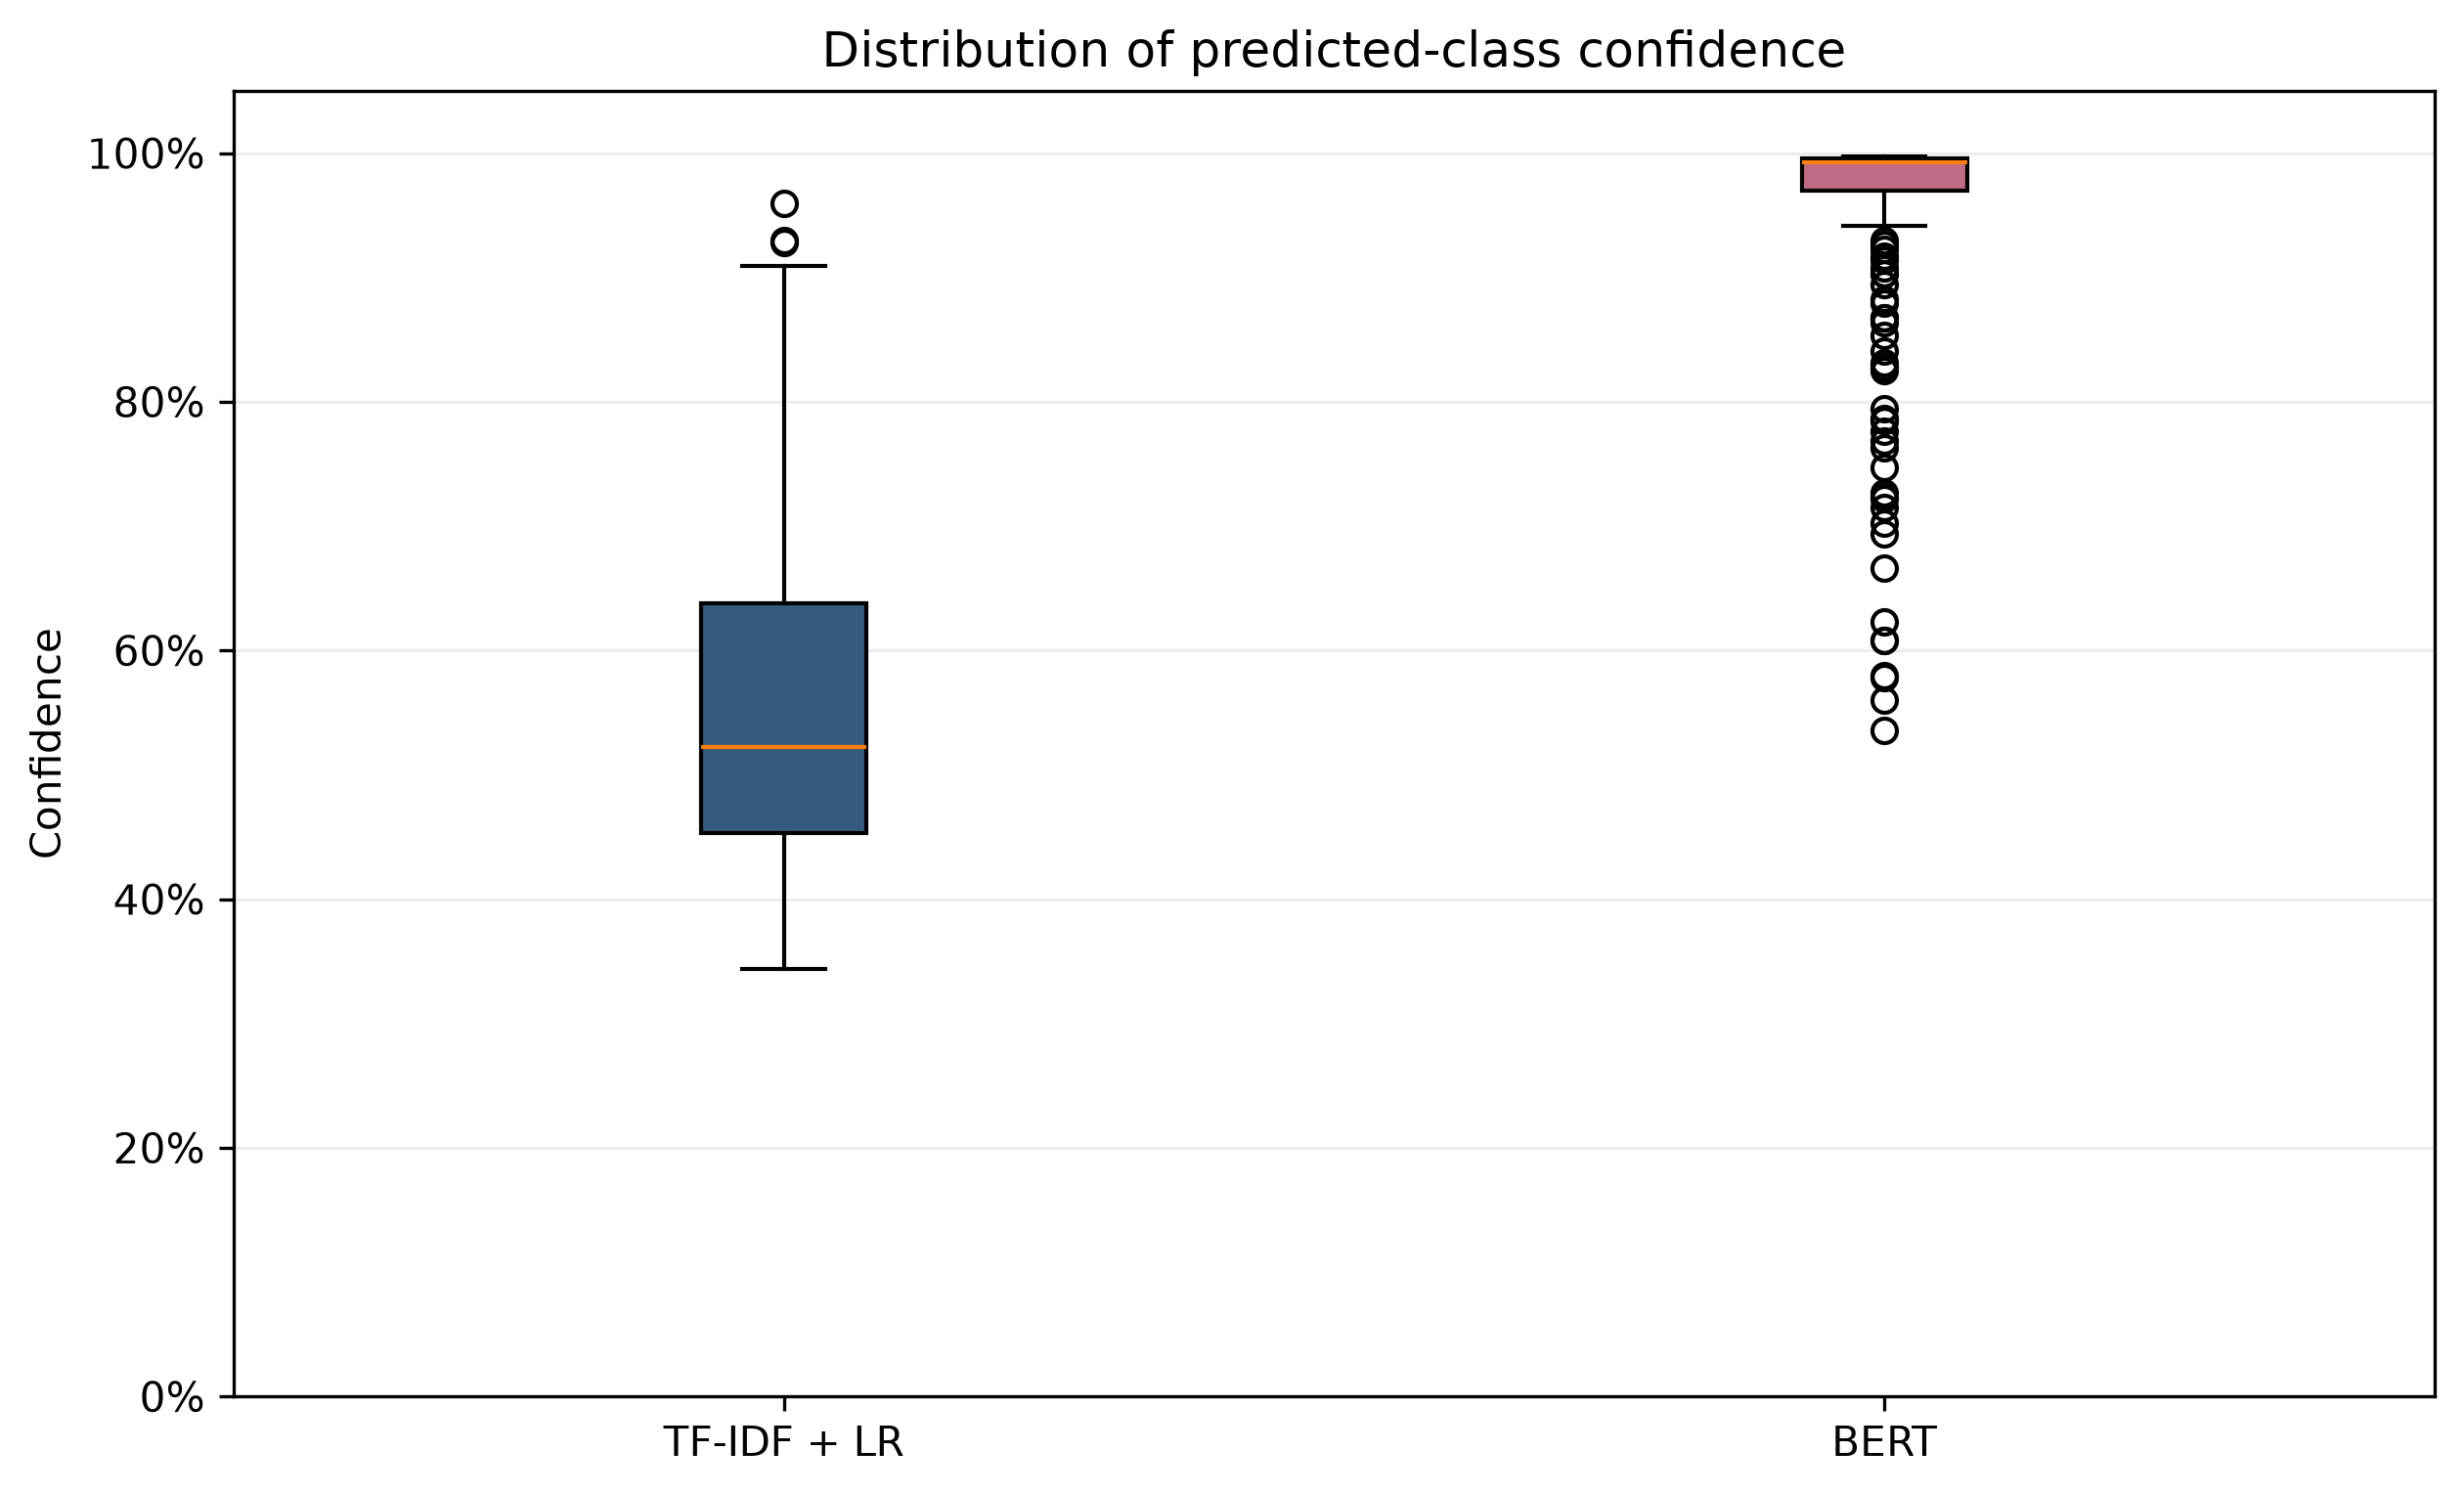
\includegraphics[width=\textwidth]{confidence_distribution.png}
\end{subfigure}
\hfill
\begin{subfigure}[b]{0.48\textwidth}
\centering
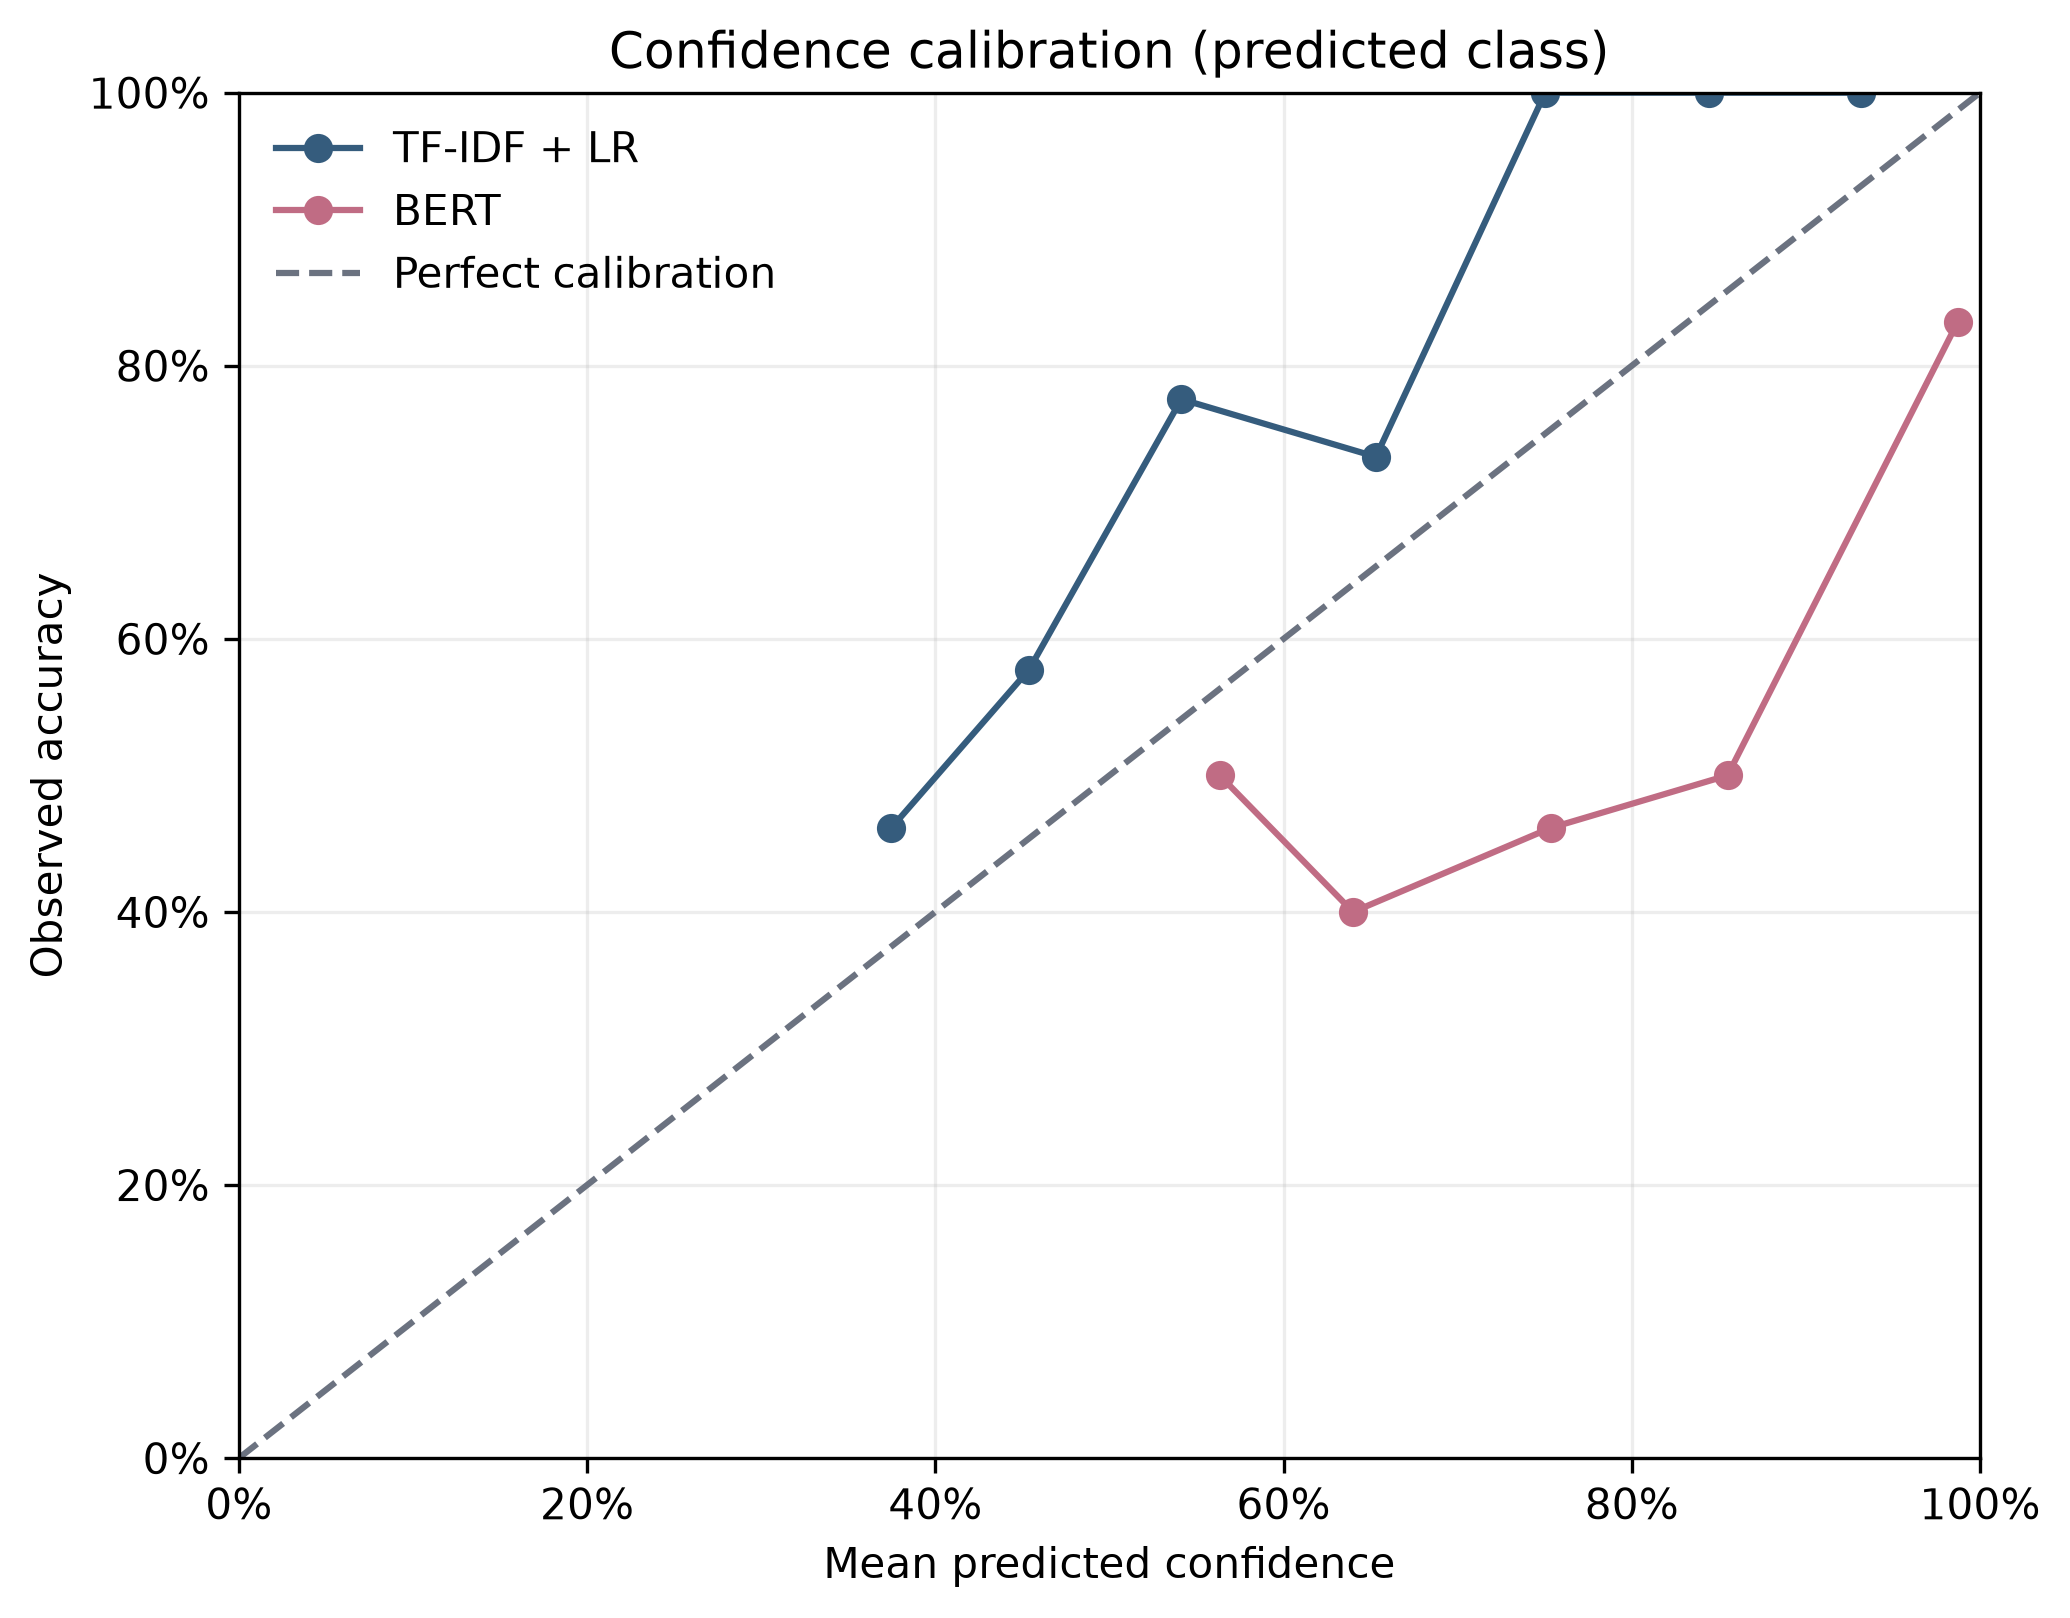
\includegraphics[width=\textwidth]{calibration.png}
\end{subfigure}
\caption{Confidence distribution (left) and calibration reliability diagram against the perfect-calibration diagonal (right).}
\end{figure}

Despite far higher average confidence, BERT's ECE (0.1767) is \emph{higher}, not lower, than TF-IDF's (0.1554): BERT's confidence outpaces its accuracy by a wider margin than TF-IDF's does, consistent with systematic overconfidence in BERT's high-confidence bins. Confidence is not accuracy --- BERT's 94.60\% mean confidence does not imply 94.60\% accuracy; its measured accuracy on this test set is 76.92\%.

\begin{figure}[H]
\centering
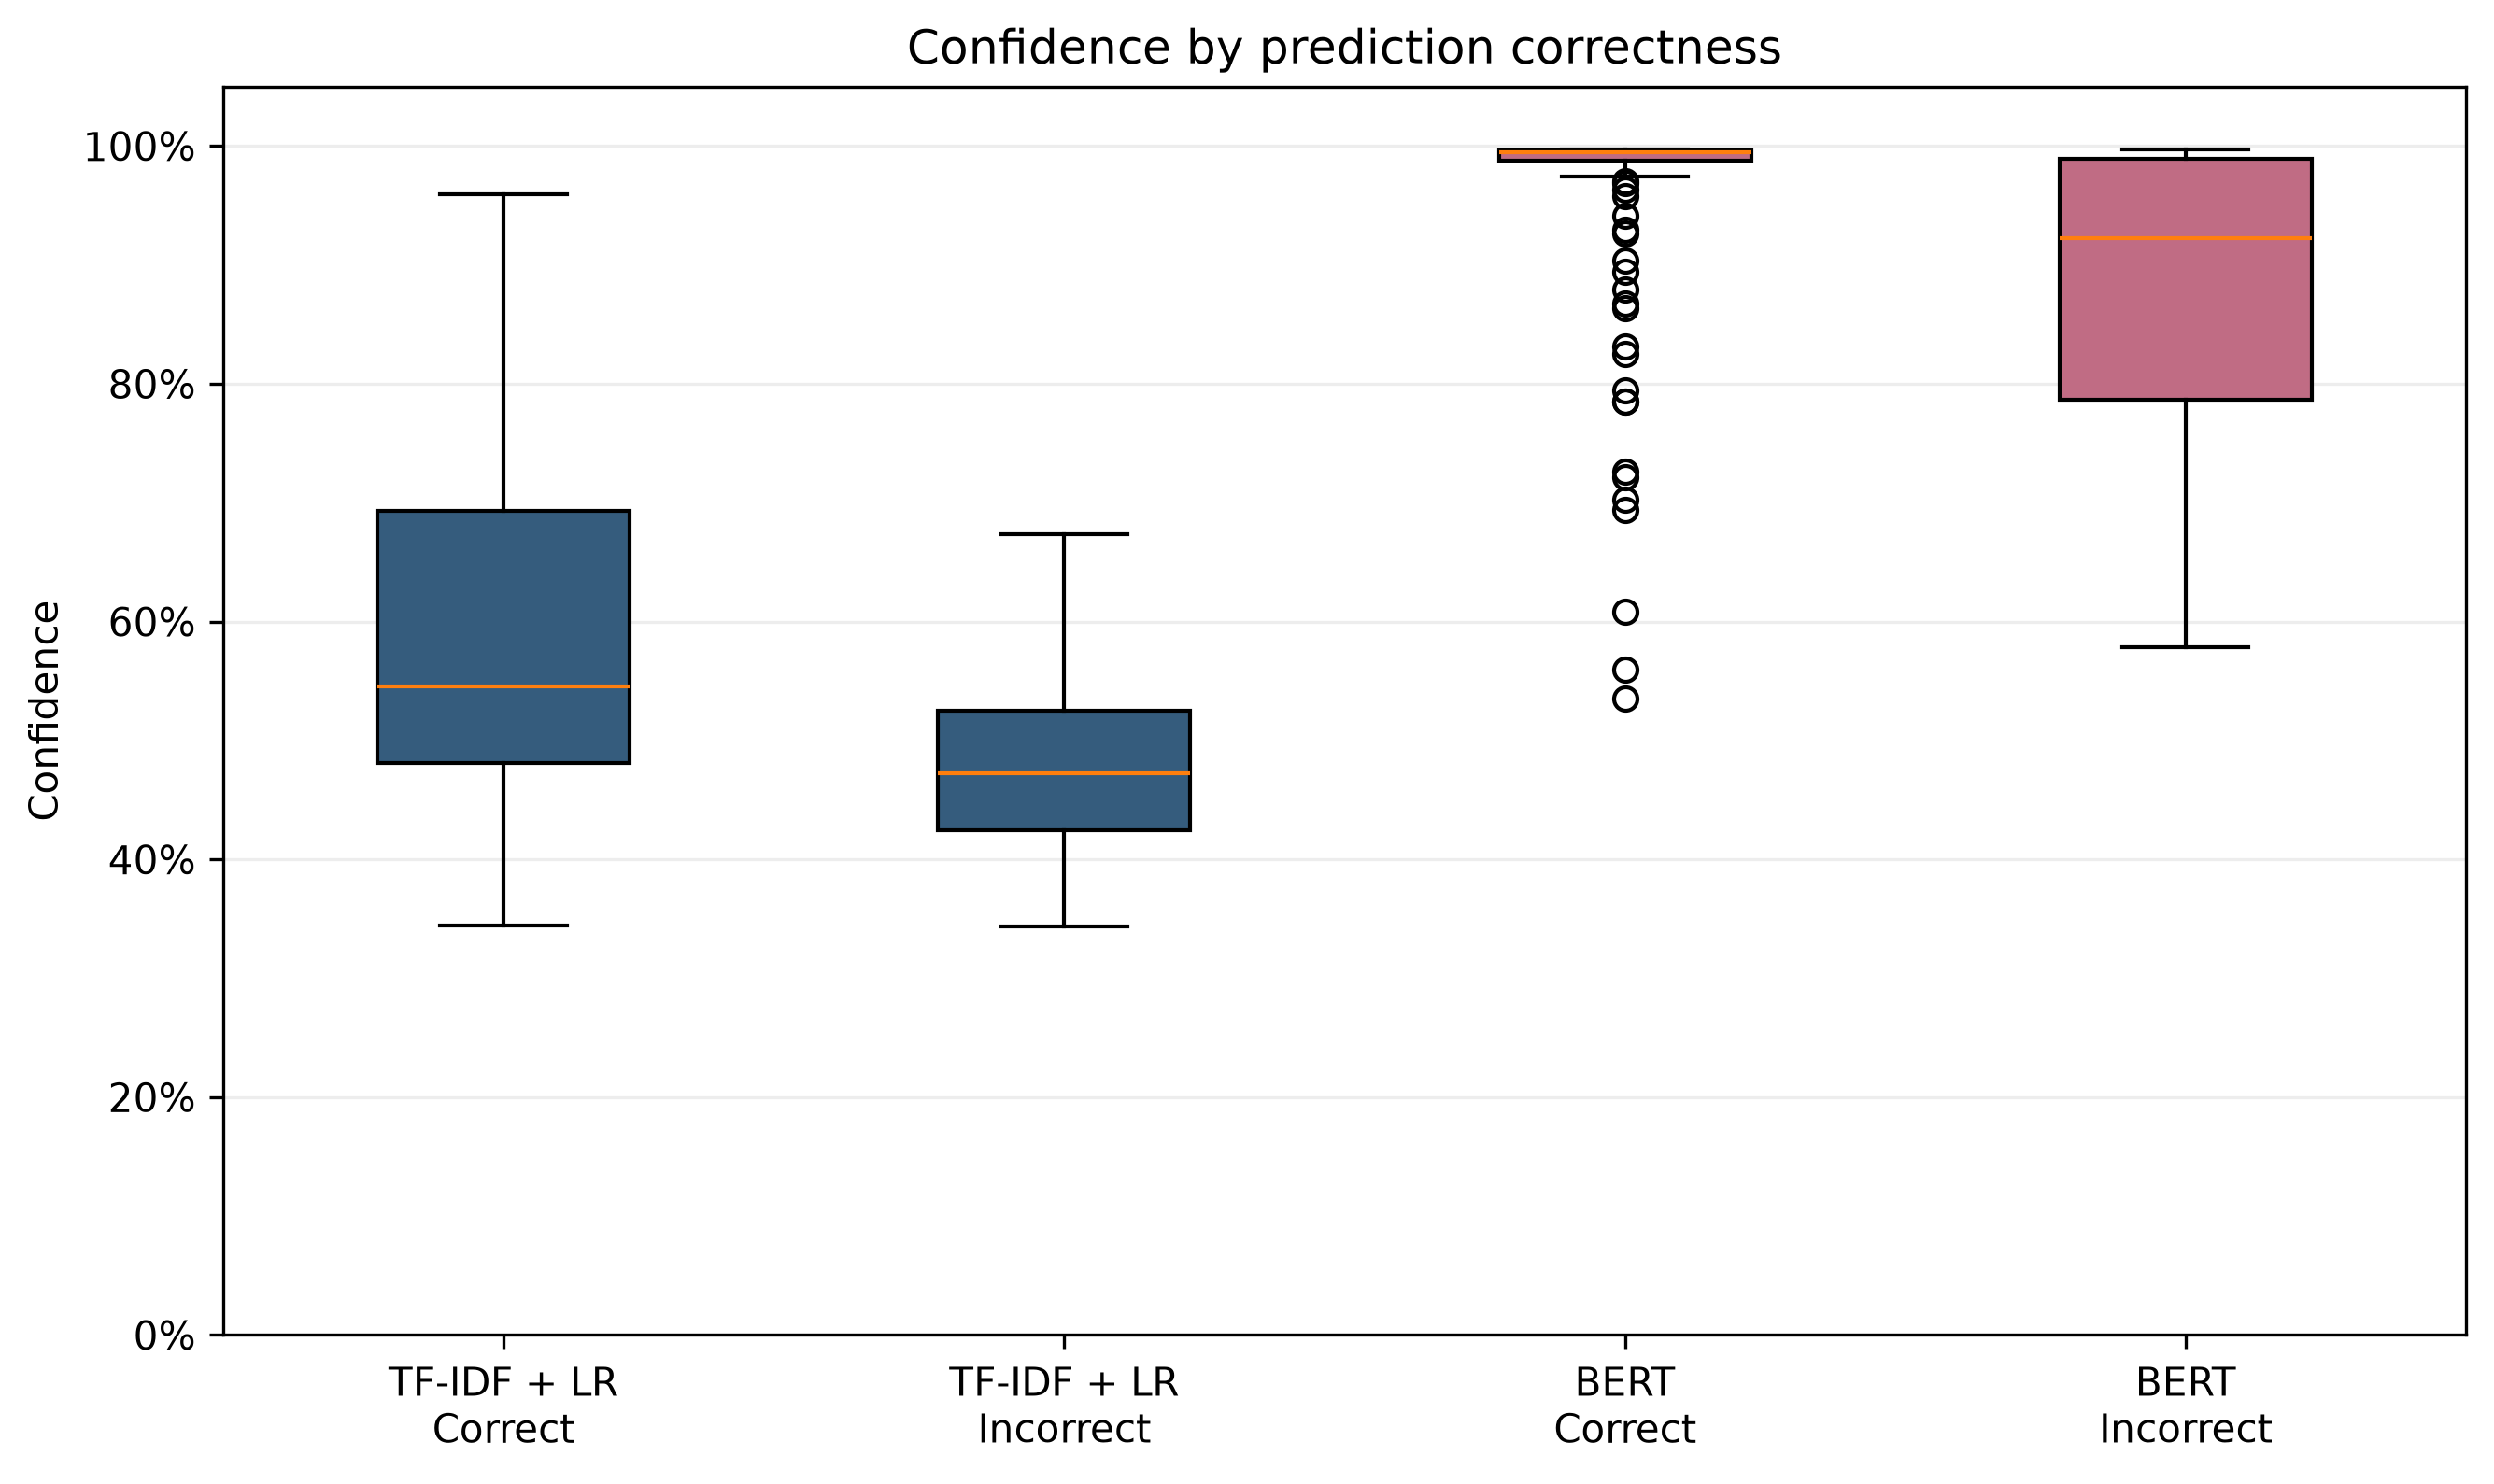
\includegraphics[width=0.7\textwidth]{confidence_vs_correctness.png}
\caption{Selected-class confidence, grouped by model and by prediction correctness.}
\end{figure}

For both models, correct predictions carry higher confidence than incorrect ones, the expected direction for a usable signal. But because BERT's confidence is compressed near 1.0 even for many incorrect predictions, a fixed high-confidence threshold on BERT would still pass a non-trivial share of wrong answers; TF-IDF's more spread confidence is comparatively more informative per example, even though its overall accuracy is lower.

\subsection{Agreement}

\begin{table}[H]
\centering
\caption{Model agreement on the 195-row test set.}
\begin{tabular}{lrr}
\toprule
\textbf{Outcome} & \textbf{Count} & \textbf{Share} \\
\midrule
Agreement    & 148 & 75.9\% \\
Disagreement & 47  & 24.1\% \\
\bottomrule
\end{tabular}
\end{table}

\begin{figure}[H]
\centering
\begin{subfigure}[b]{0.48\textwidth}
\centering
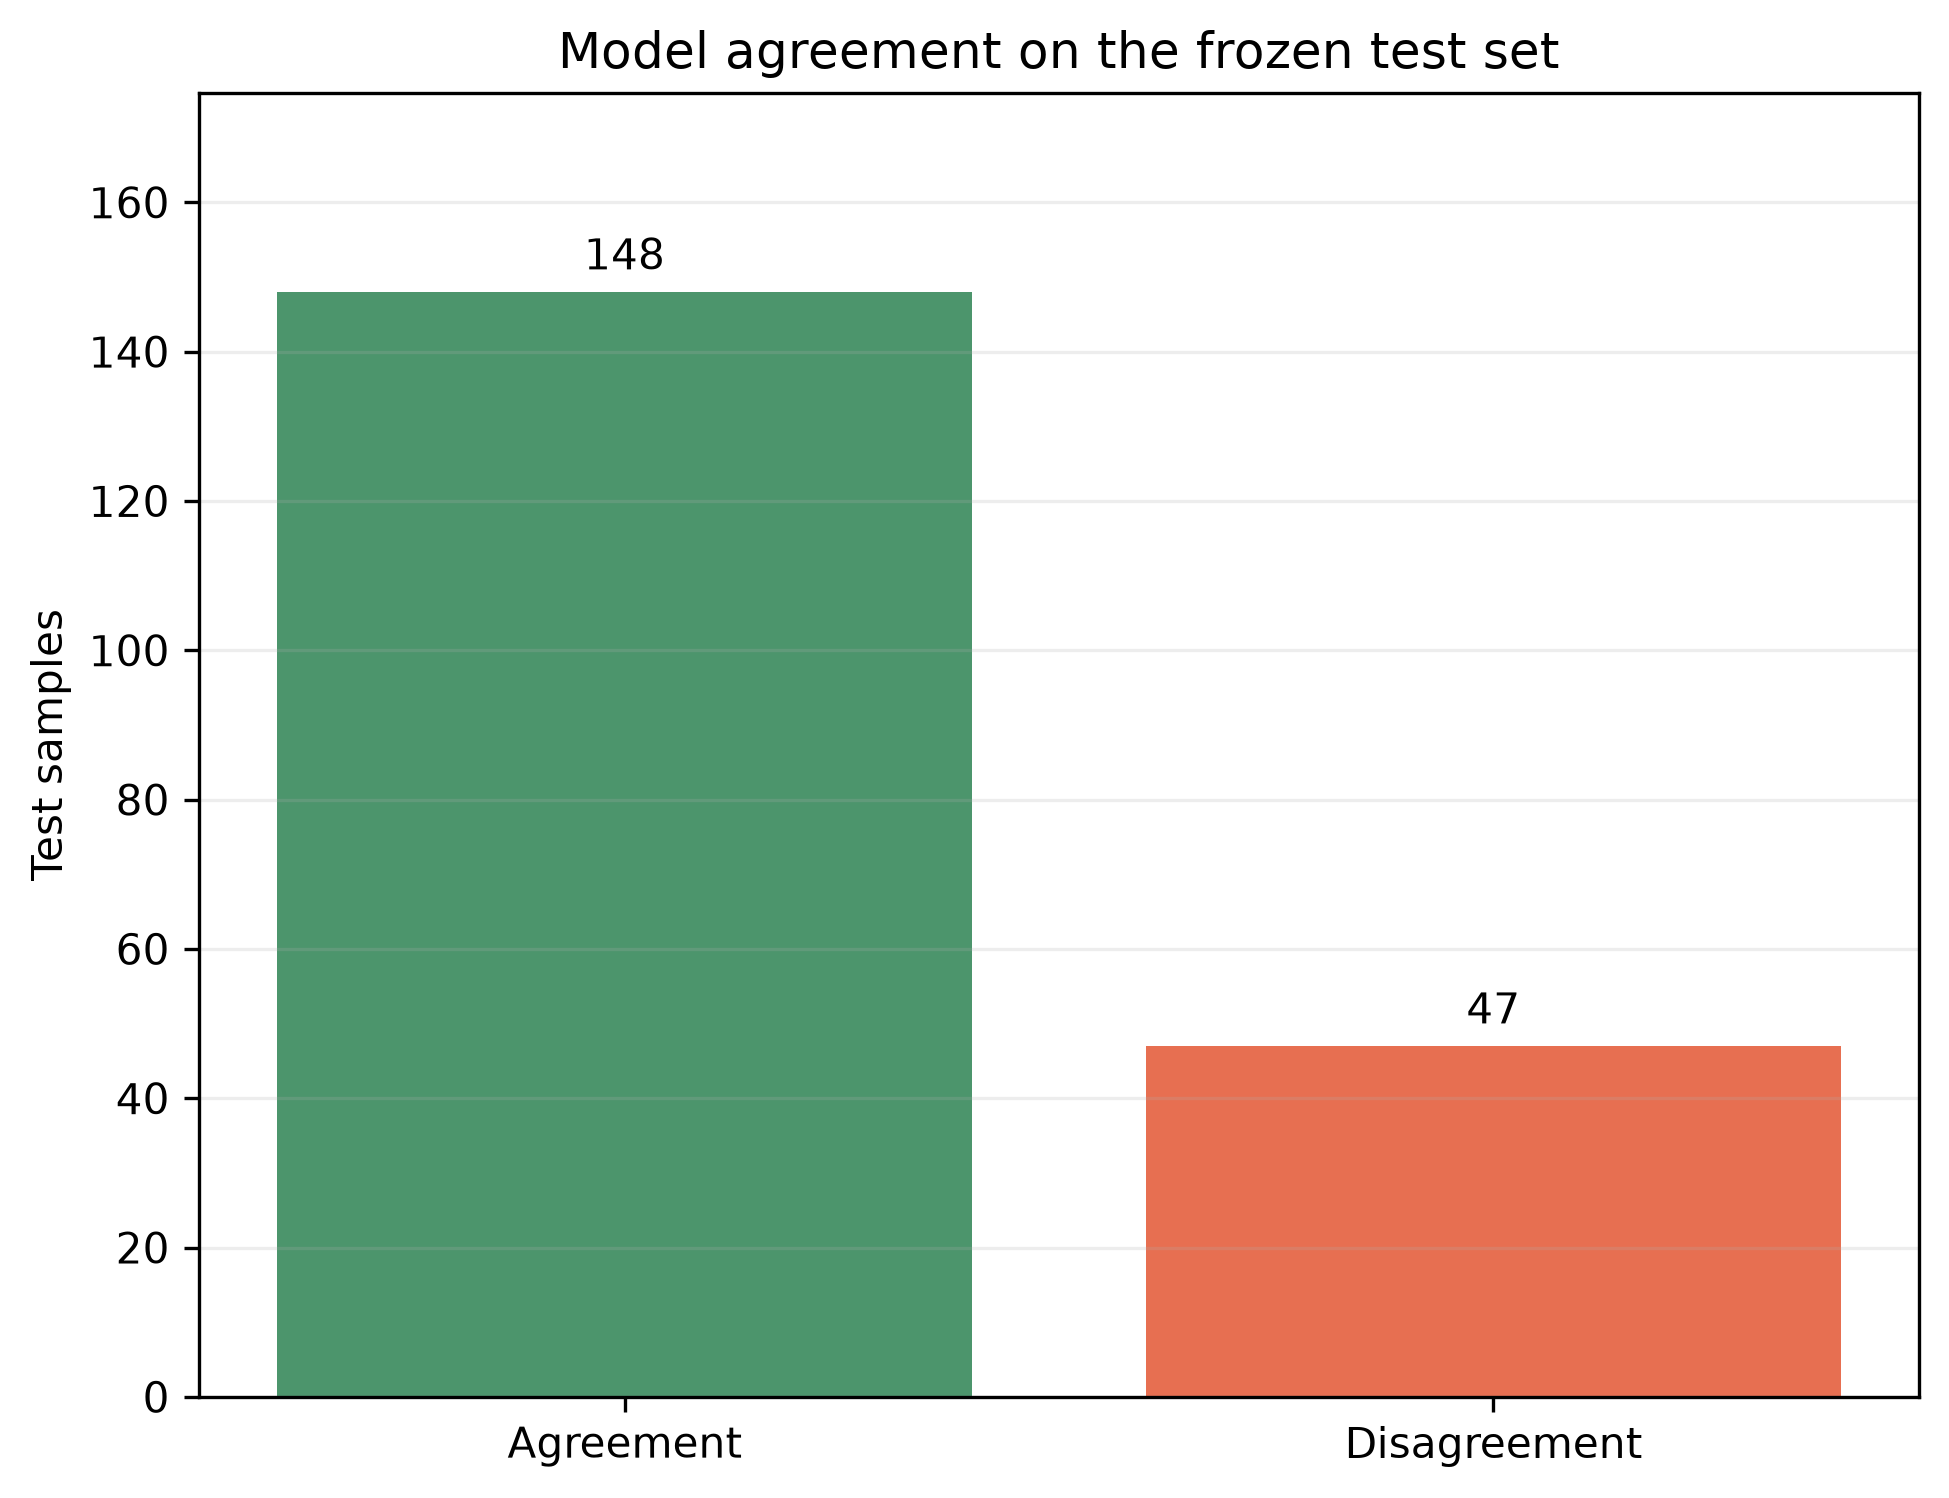
\includegraphics[width=\textwidth]{model_agreement.png}
\end{subfigure}
\hfill
\begin{subfigure}[b]{0.48\textwidth}
\centering
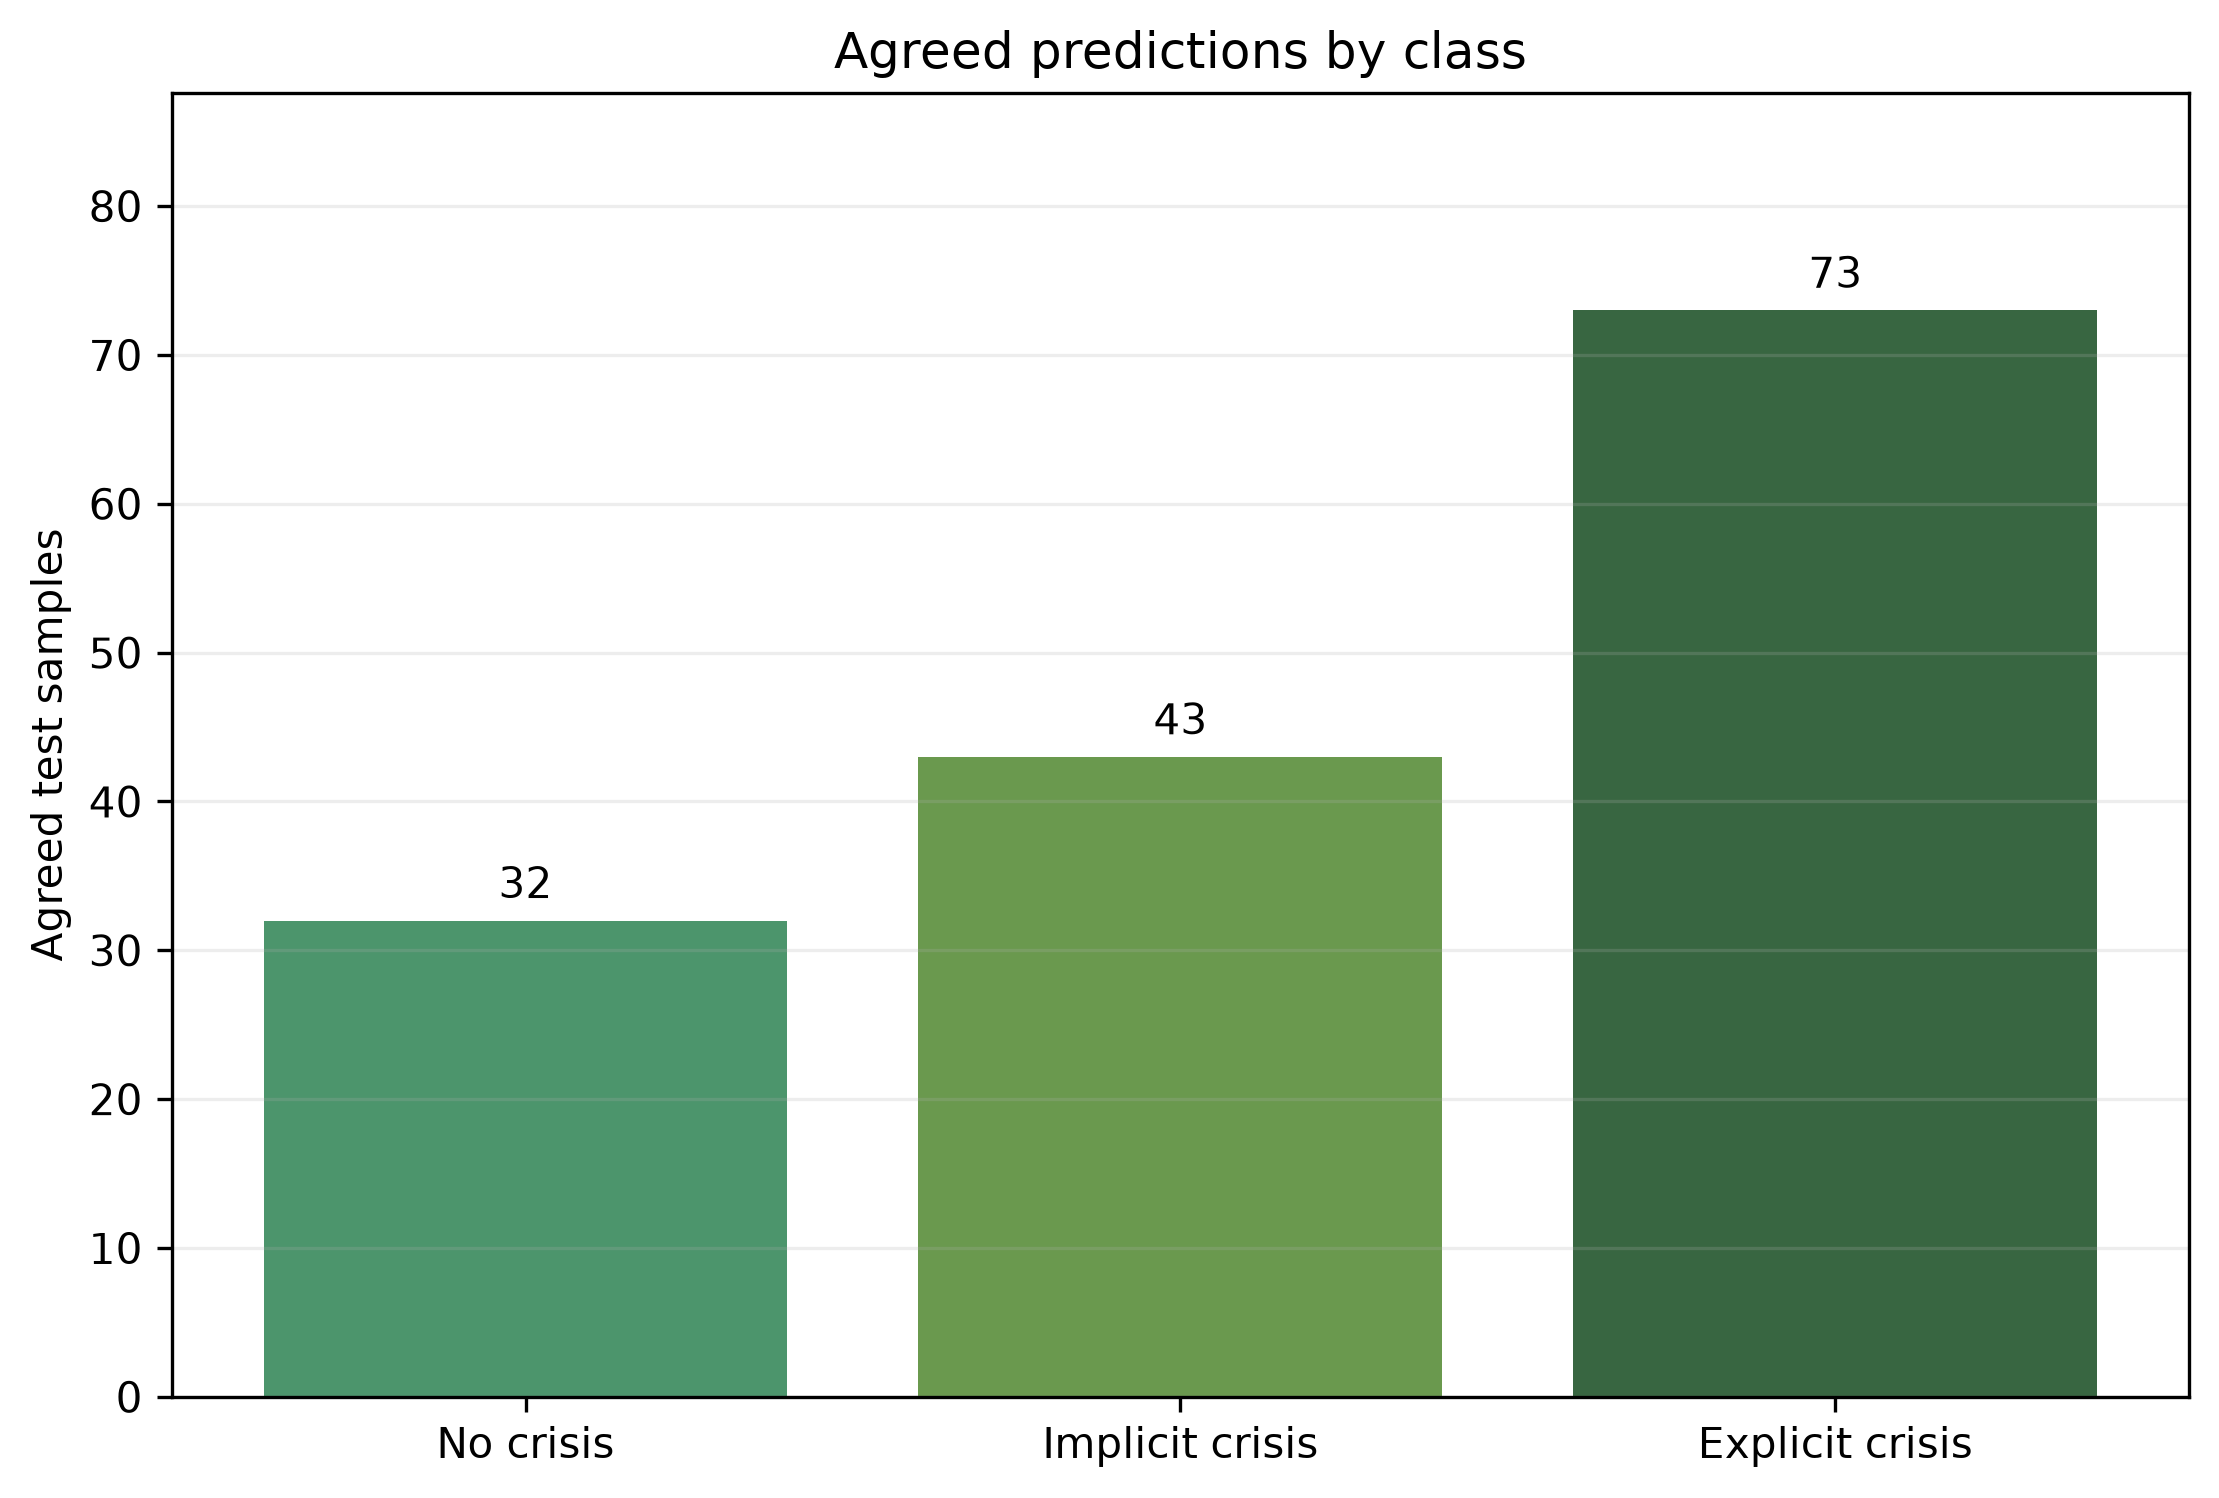
\includegraphics[width=\textwidth]{agreement_by_class.png}
\end{subfigure}
\caption{Overall agreement/disagreement counts (left) and class distribution among agreeing predictions (right).}
\end{figure}

\begin{figure}[H]
\centering
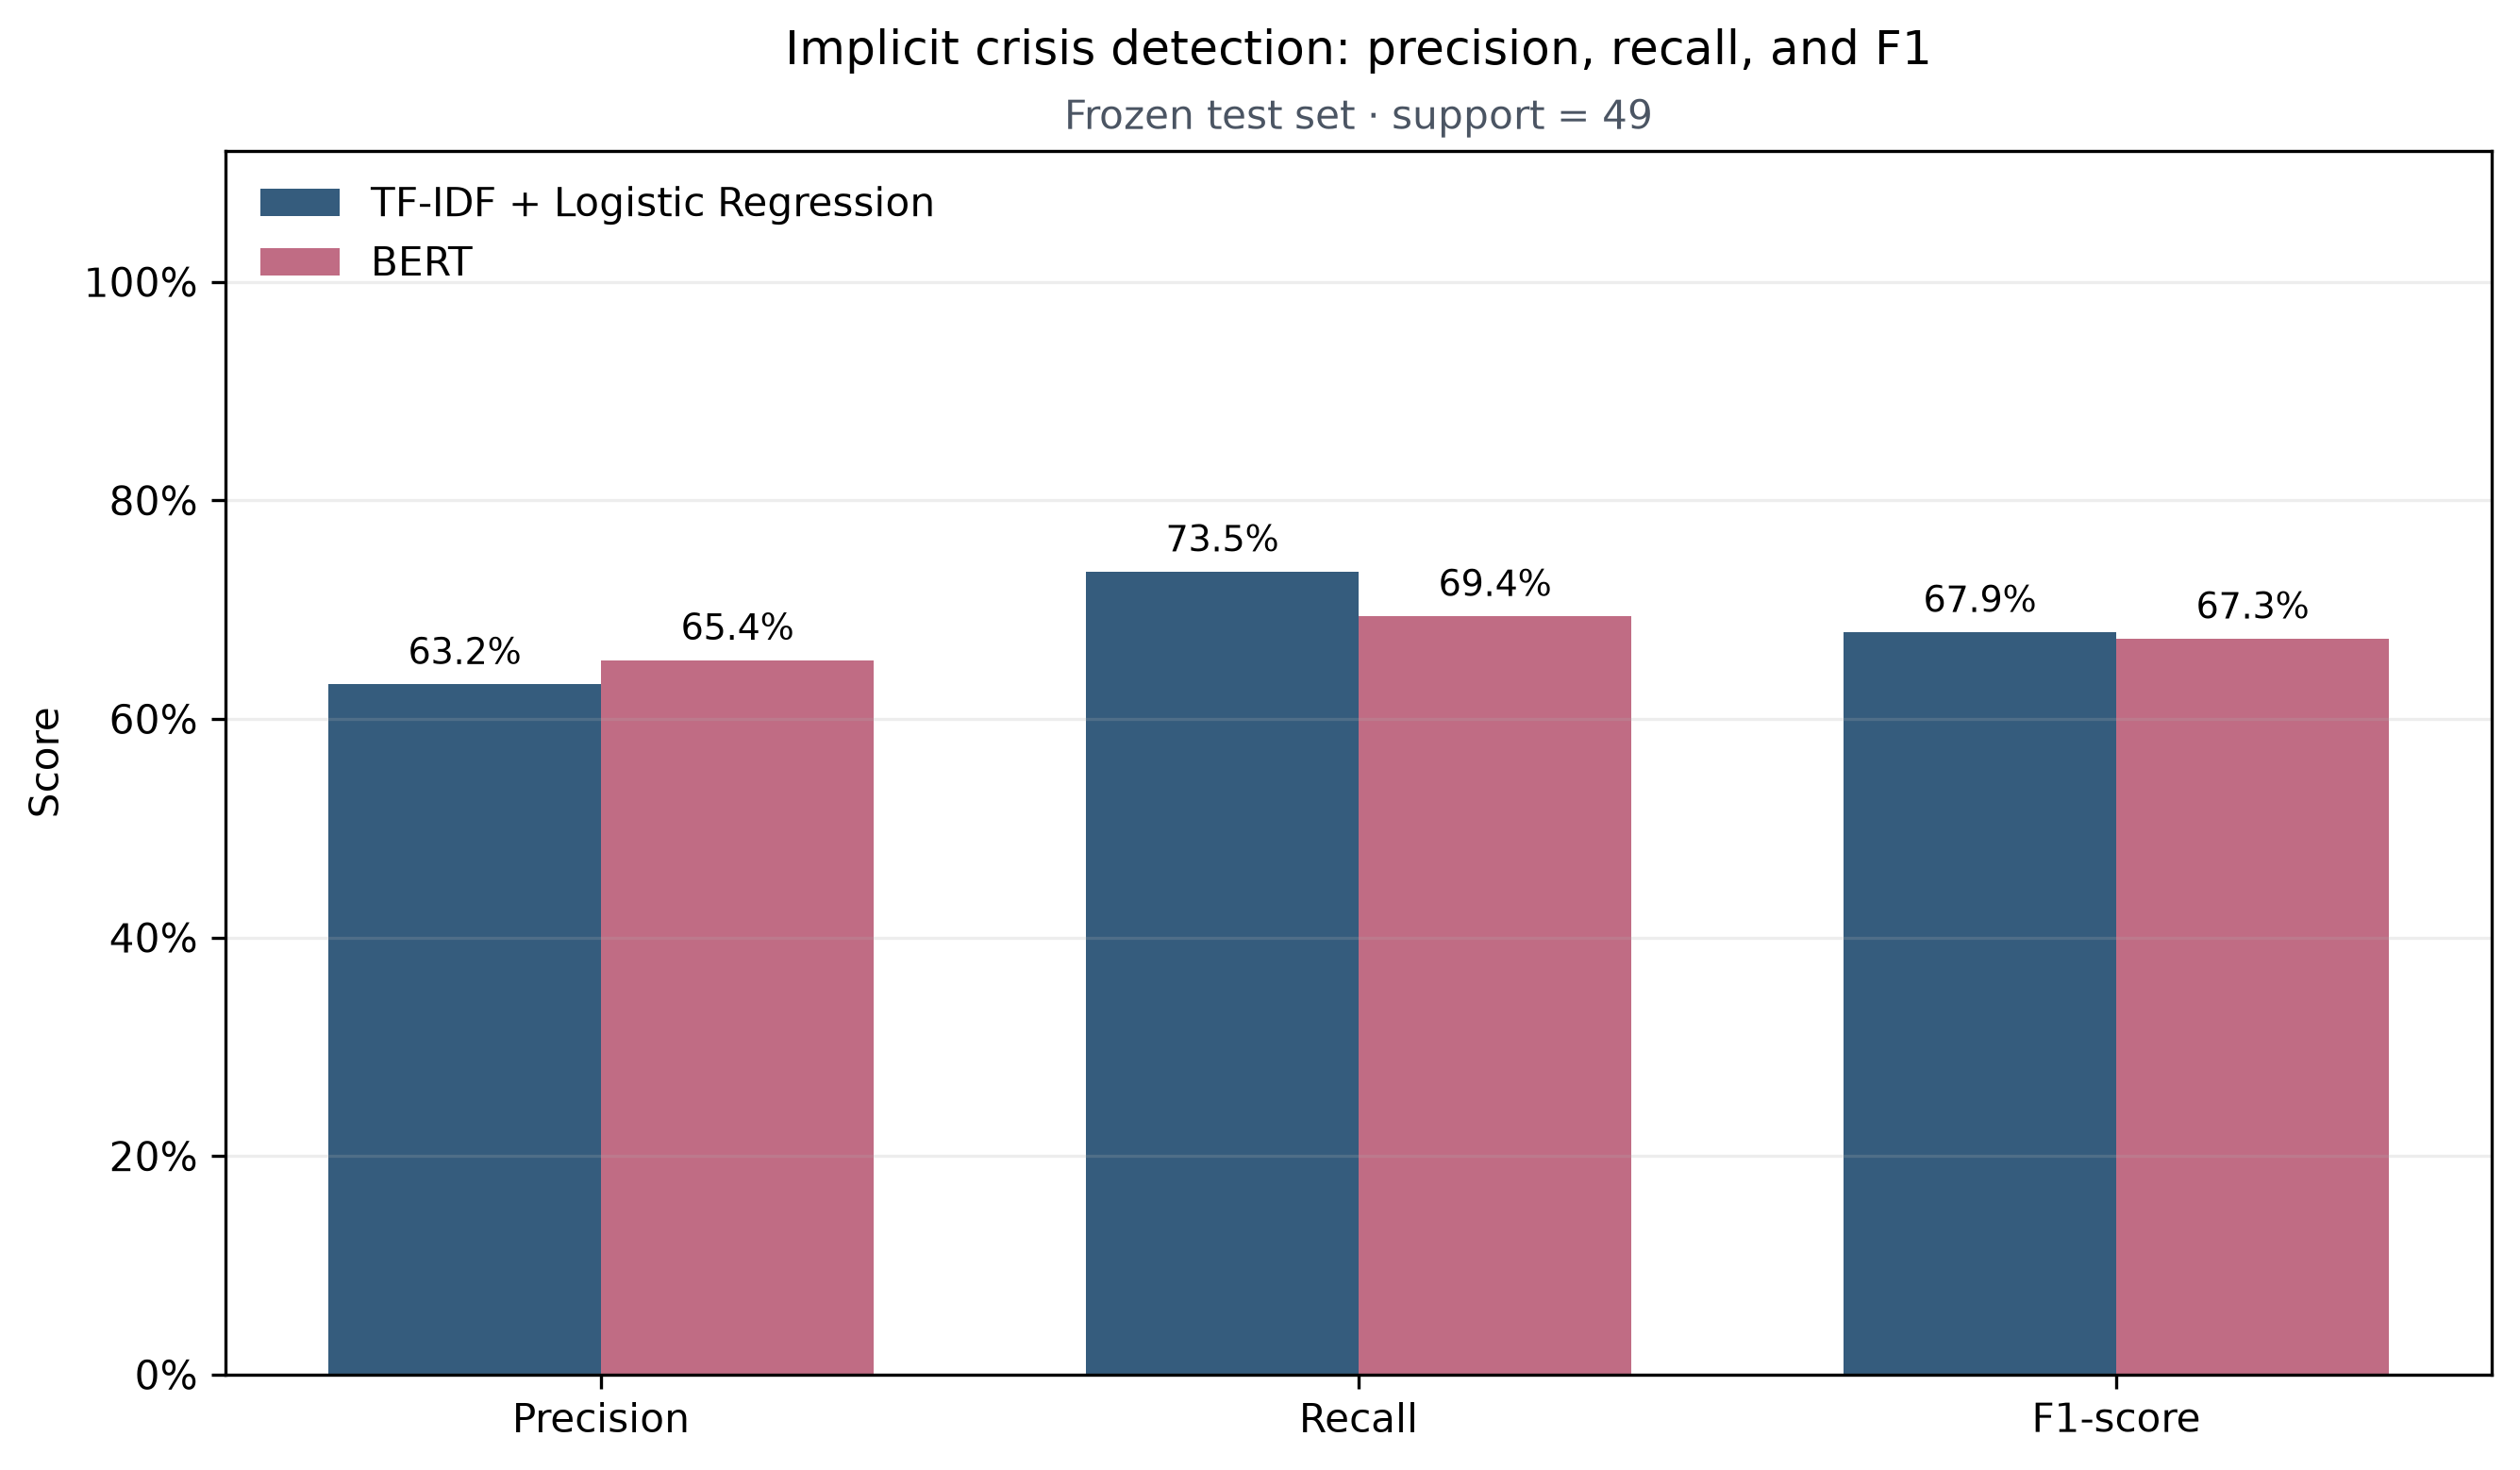
\includegraphics[width=0.65\textwidth]{implicit_crisis_metrics.png}
\caption{Implicit-crisis-specific metric comparison between TF-IDF + Logistic Regression and BERT.}
\end{figure}

Agreement means both independently trained models selected the same label; it says nothing about whether that label is correct. Of the 195 rows, both models are correct on 124 (63.6\%), both are wrong on 30 (15.4\%), TF-IDF alone is correct on 15 (7.7\%), and BERT alone is correct on 26 (13.3\%). BERT is uniquely correct on roughly 1.7$\times$ as many rows as TF-IDF is uniquely correct on, but the existence of 15 TF-IDF-only-correct rows shows the lexical model is not strictly subsumed by the transformer.

\subsection{Error Analysis}

From \texttt{predictions.csv} (195 rows): no-crisis$\rightarrow$explicit-crisis errors occur on 13/53 no-crisis rows for TF-IDF versus 5/53 for BERT; explicit-crisis$\rightarrow$no-crisis errors occur on 9/93 for TF-IDF versus 7/93 for BERT; implicit-crisis confusion with no-crisis is identical for both models (4/49), while TF-IDF confuses implicit-crisis with explicit-crisis slightly less often than BERT (9/49 vs.\ 11/49). The pattern is not that one model is strictly superior: BERT more effectively separates no-crisis from explicit-crisis text, but the two models are essentially interchangeable on implicit-crisis, and each correctly classifies a non-overlapping subset of examples the other gets wrong.

\subsection{Discussion}

\textbf{Overall comparison.} On this frozen 195-sample set, BERT achieves higher overall accuracy and macro-F1, while TF-IDF + Logistic Regression achieves slightly higher implicit-crisis F1. Neither model is uniformly superior across every axis measured; the correct framing is comparative and class-conditional, not a single ``which model wins'' verdict.

\textbf{Implicit crisis is the hard class for both models.} Both models score worst, relative to their own explicit-crisis performance, on implicit-crisis (TF-IDF: 67.9\% vs.\ 77.0\%; BERT: 67.3\% vs.\ 84.7\%). That BERT's added contextual capacity does not clearly beat the much simpler TF-IDF baseline here is the most notable finding of this comparison, suggesting the gap between implicit and explicit crisis language is not primarily one that more contextual power alone closes.

\textbf{Confidence is not a reliability signal by itself.} BERT's much higher confidence, paired with a higher ECE, means any downstream use of confidence (e.g., flagging low-confidence predictions for review) needs model-specific thresholds; a fixed threshold does not carry equal meaning for both models.

\textbf{Agreement is not correctness.} The two models disagree on 24.1\% of rows, and TF-IDF is uniquely correct on 15 of those --- disagreement does not mean the more sophisticated model is the one that is right.

\textbf{Practical interpretation.} These results support presenting both models' predictions side by side, as CrisisSense's frontend does, rather than treating either model as a ground-truth signal or combining them into a single ensemble score that would obscure exactly the class-conditional and confidence-conditional differences documented above. A practitioner interested specifically in implicit-crisis recall should not assume that deploying only the larger, higher-accuracy model is sufficient; the evidence here suggests the two models are close to interchangeable on that specific class.

\textbf{What these results do and do not show.} These results show: (1) BERT's higher accuracy and macro-F1 on this specific 195-row test set; (2) an approximate tie between the two models on implicit-crisis F1; (3) that BERT's much higher confidence is accompanied by somewhat worse calibration, not better; and (4) that model agreement does not imply correctness for either model. They do \emph{not} show that BERT is unconditionally better than TF-IDF at implicit-crisis detection, that either model generalizes beyond this dataset's distribution, that either model's confidence score is directly usable as a calibrated probability without further calibration work, or that either model is suitable for any form of individual-level clinical or risk assessment.

\section{Conclusion and Limitations}

CrisisSense compares a character-level TF-IDF + Logistic Regression baseline against a frozen BERT sequence classifier on an identical 195-row test set. BERT leads on overall accuracy, macro-F1, and per-class F1 for no-crisis and explicit-crisis; TF-IDF is marginally ahead on implicit-crisis F1. BERT's much higher confidence is not accompanied by better calibration, and model agreement (75.9\%) is not evidence of correctness. Several limitations bound these conclusions:

\begin{itemize}[nosep]
  \item The test set has only 195 rows, 49 of them implicit-crisis --- the narrowest evidentiary base in this report.
  \item Both models show non-trivial ECE (0.155--0.177); neither model's raw softmax probability is a calibrated estimate of correctness.
  \item Both models are frozen inference-only artifacts; BERT's original fine-tuning run is not re-executed or re-verified here.
  \item Results are scoped to this dataset's distribution; generalization to other platforms, writing styles, or time periods is untested.
  \item CrisisSense performs text classification only. It does not diagnose individuals, does not assess suicide risk, and is not a clinical tool.
\end{itemize}

Future work should prioritize a larger implicit-crisis-focused evaluation set, post-hoc calibration (e.g., temperature scaling) for BERT, targeted data collection around the recurring confusion patterns identified in Section~7.6, and testing on text from sources outside the current dataset's collection process.

\bibliographystyle{plain}
\bibliography{references}

\end{document}
